\section{Individual sources of Jet Energy Correction uncertainties}
\label{sec:JECs}
\begin{figure}[!hbtp]
%\begin{center}
\hspace*{-5mm}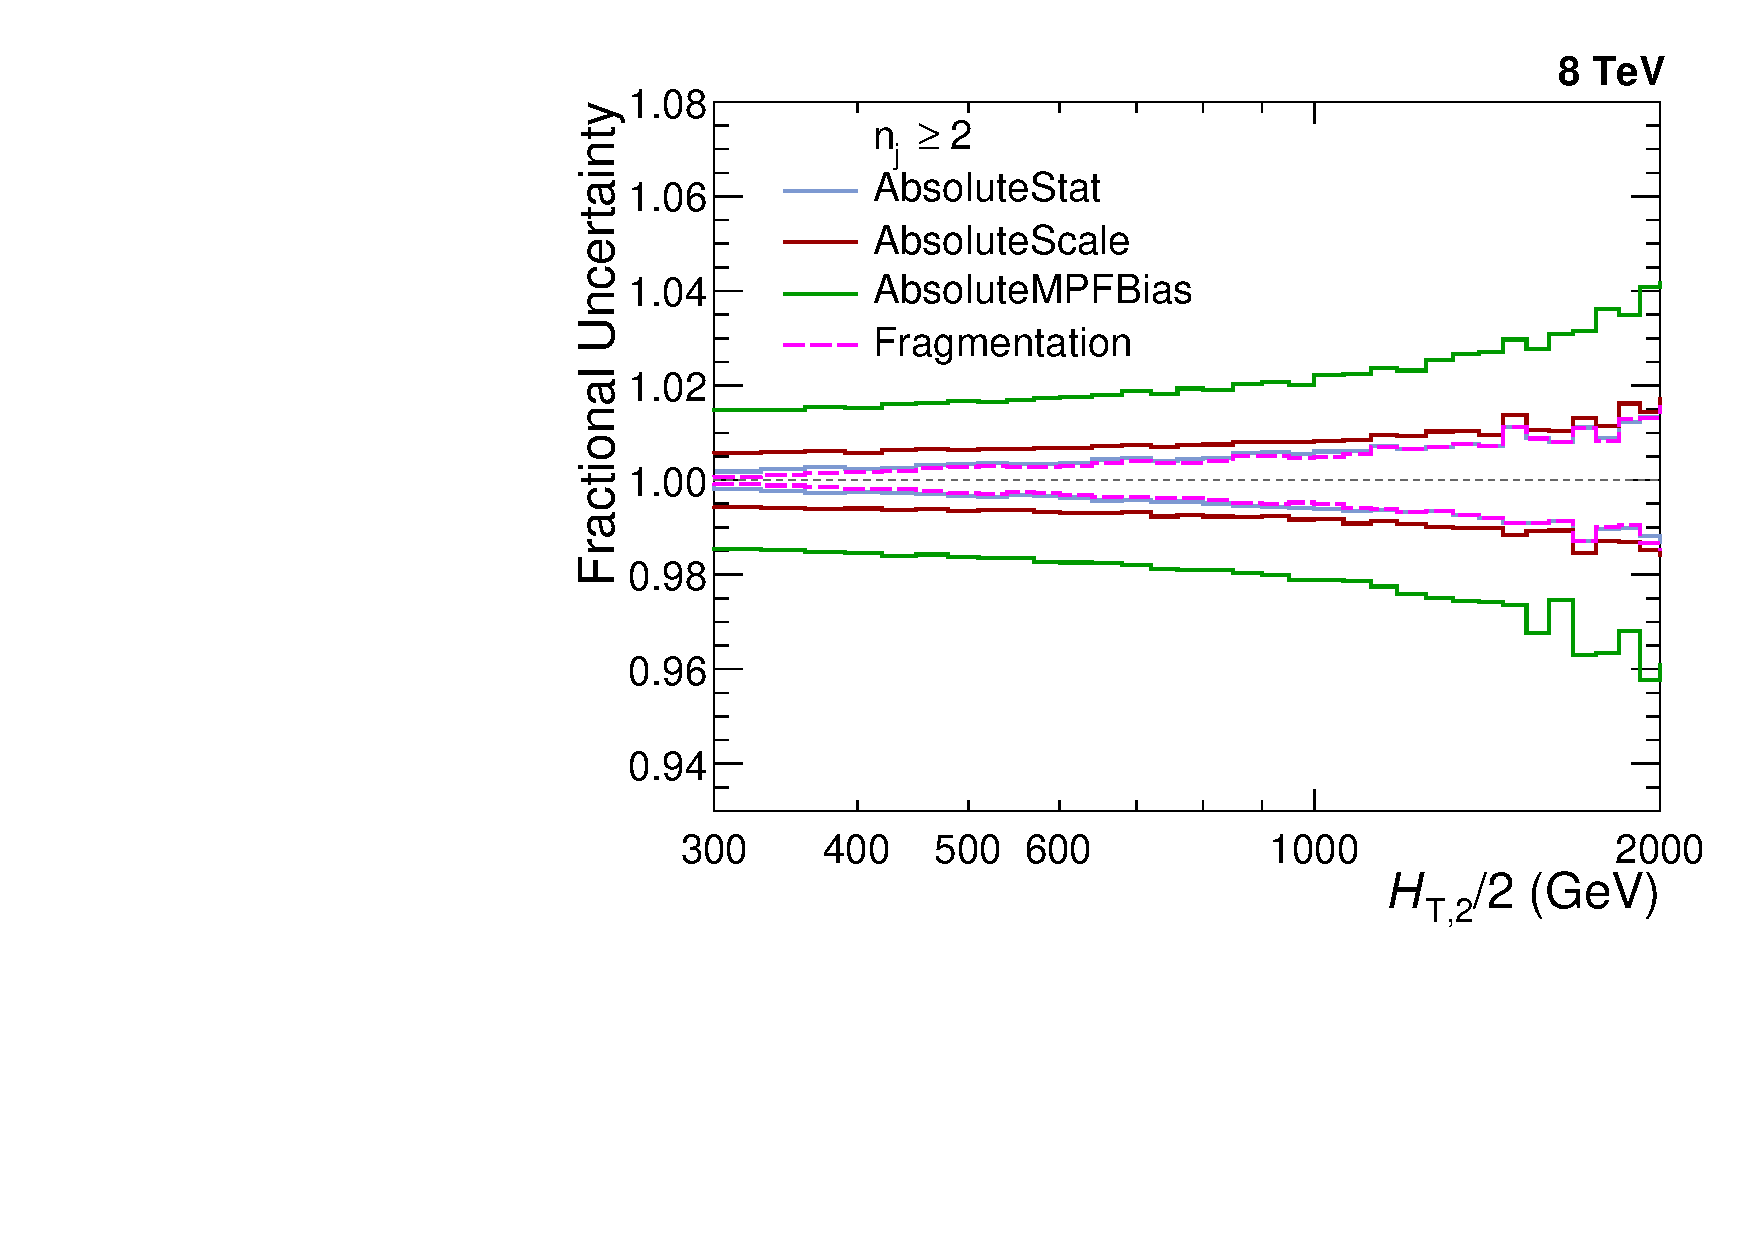
\includegraphics[width=0.51\textwidth]{/home/anter/Desktop/Thesis/Plots_HT_2_150/Single/MC_Macro_Plot_All_2_HT_2_Unc_Abs_1.pdf}%
~~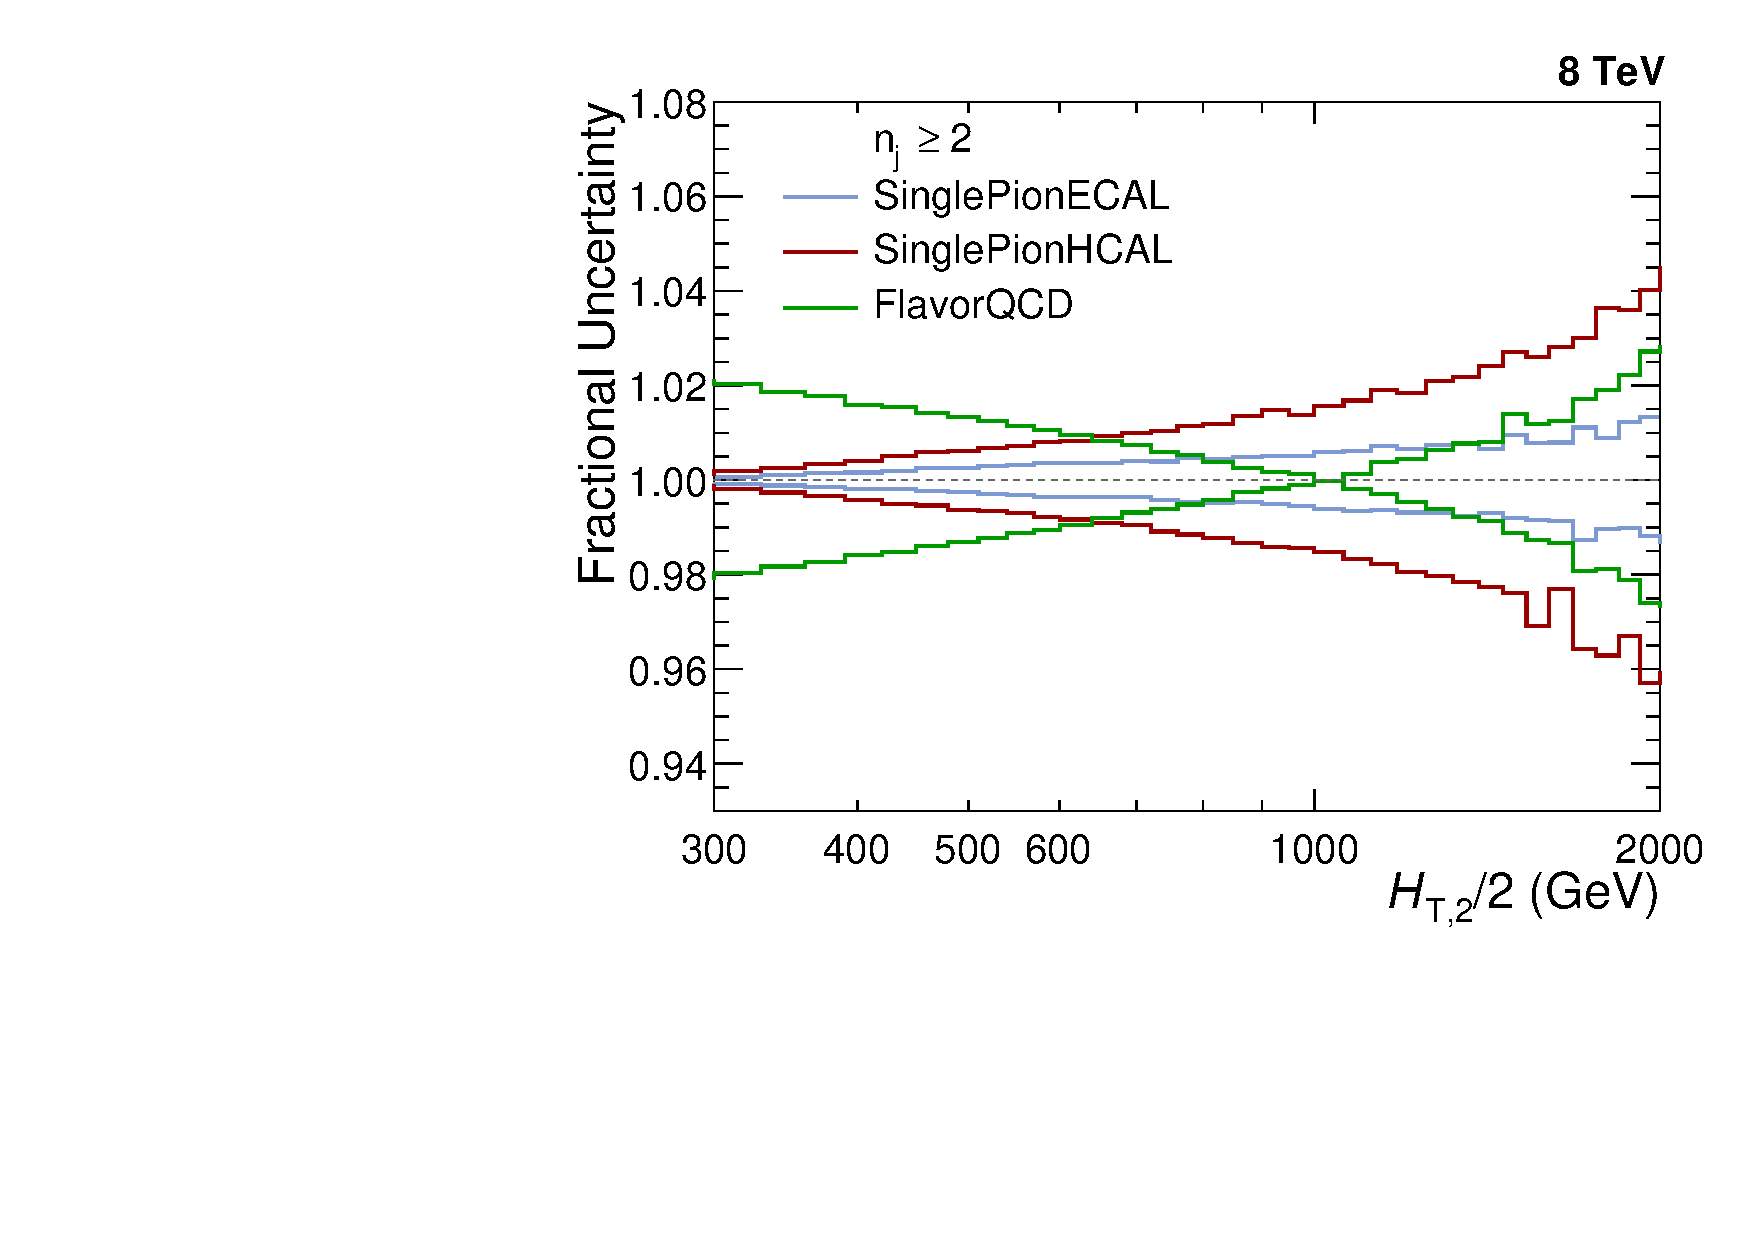
\includegraphics[width=0.51\textwidth]{/home/anter/Desktop/Thesis/Plots_HT_2_150/Single/MC_Macro_Plot_All_2_HT_2_Unc_Single_1.pdf}\\
\hspace*{-5mm}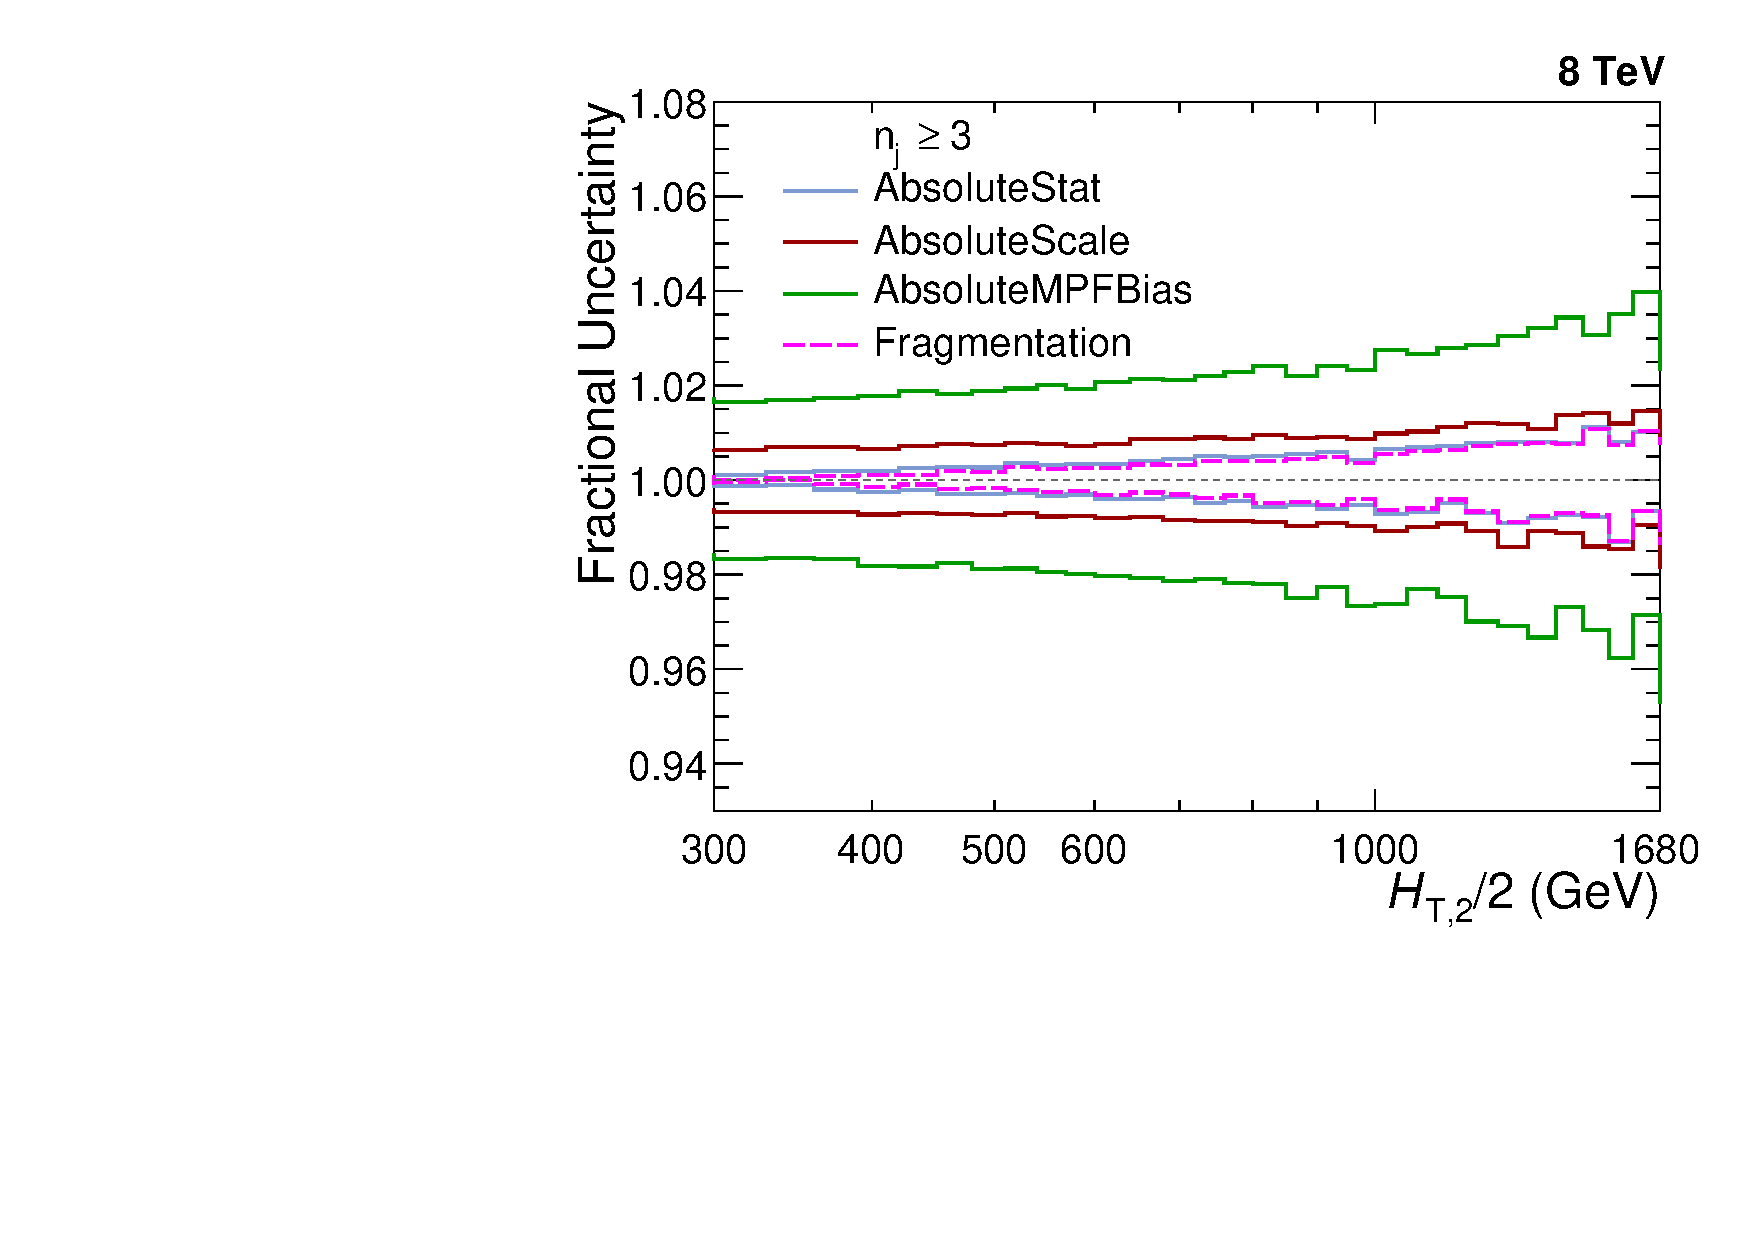
\includegraphics[width=0.51\textwidth]{/home/anter/Desktop/Thesis/Plots_HT_2_150/Single/MC_Macro_Plot_All_3_HT_2_Unc_Abs_1.pdf}%
~~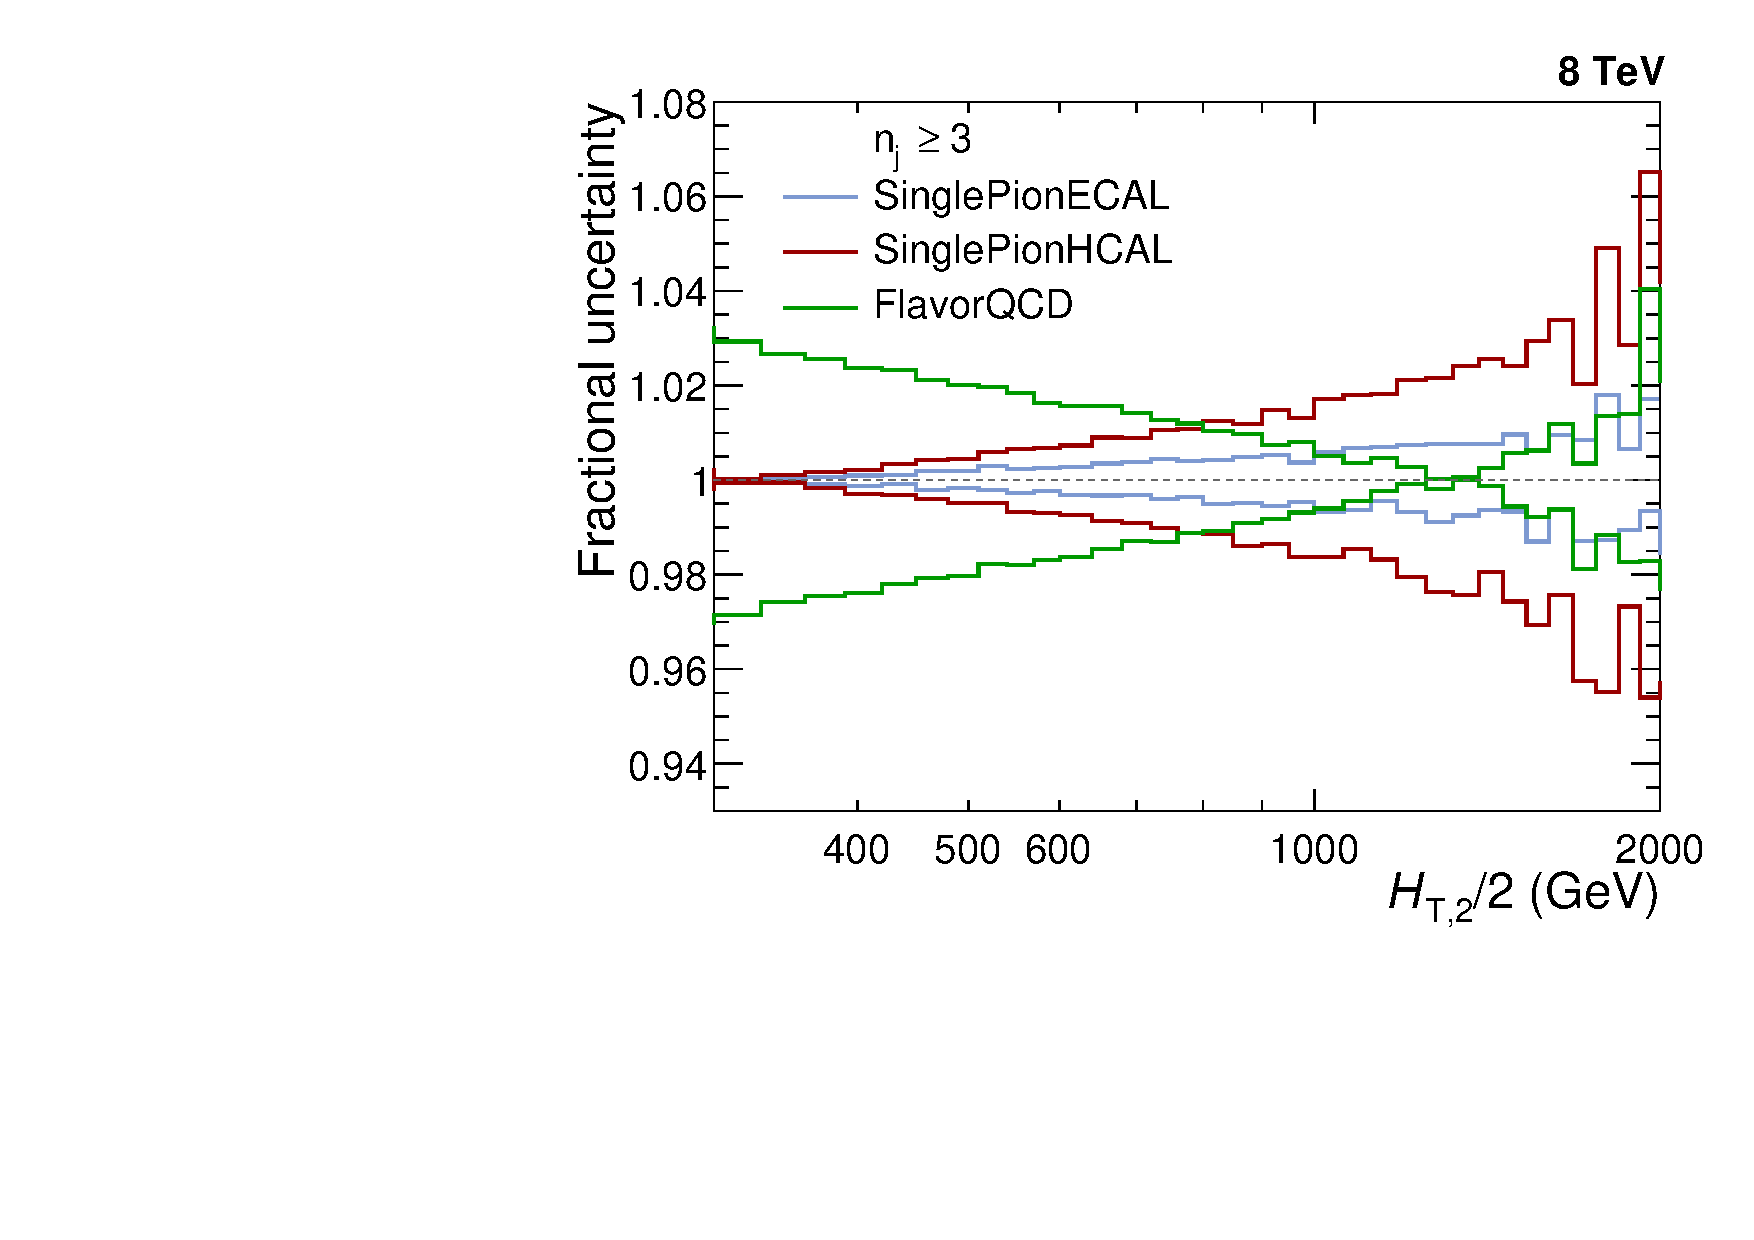
\includegraphics[width=0.51\textwidth]{/home/anter/Desktop/Thesis/Plots_HT_2_150/Single/MC_Macro_Plot_All_3_HT_2_Unc_Single_1.pdf}\\
\hspace*{-5mm}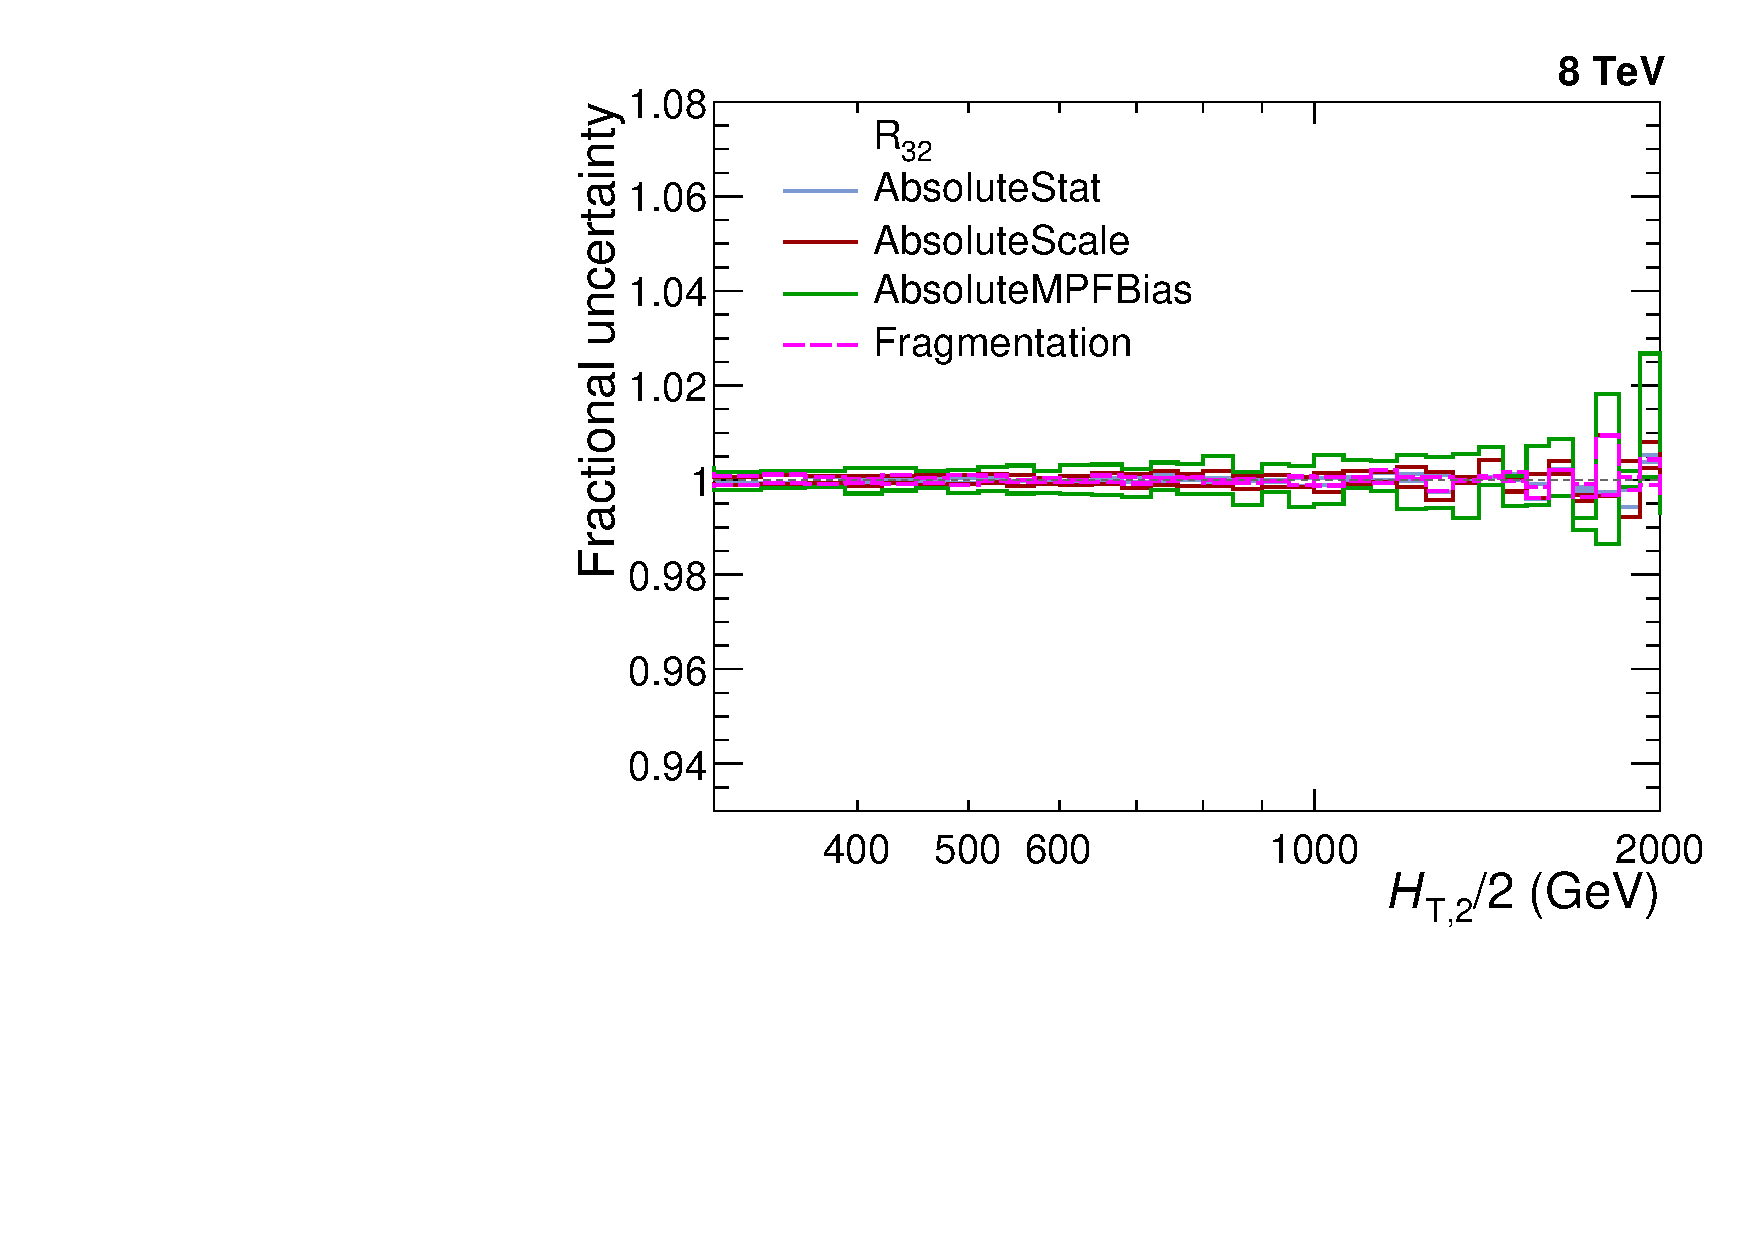
\includegraphics[width=0.51\textwidth]{/home/anter/Desktop/Thesis/Plots_HT_2_150/Single/MC_Macro_Plot_Ratio_32_HT_2_Unc_Abs_1.pdf}%
~~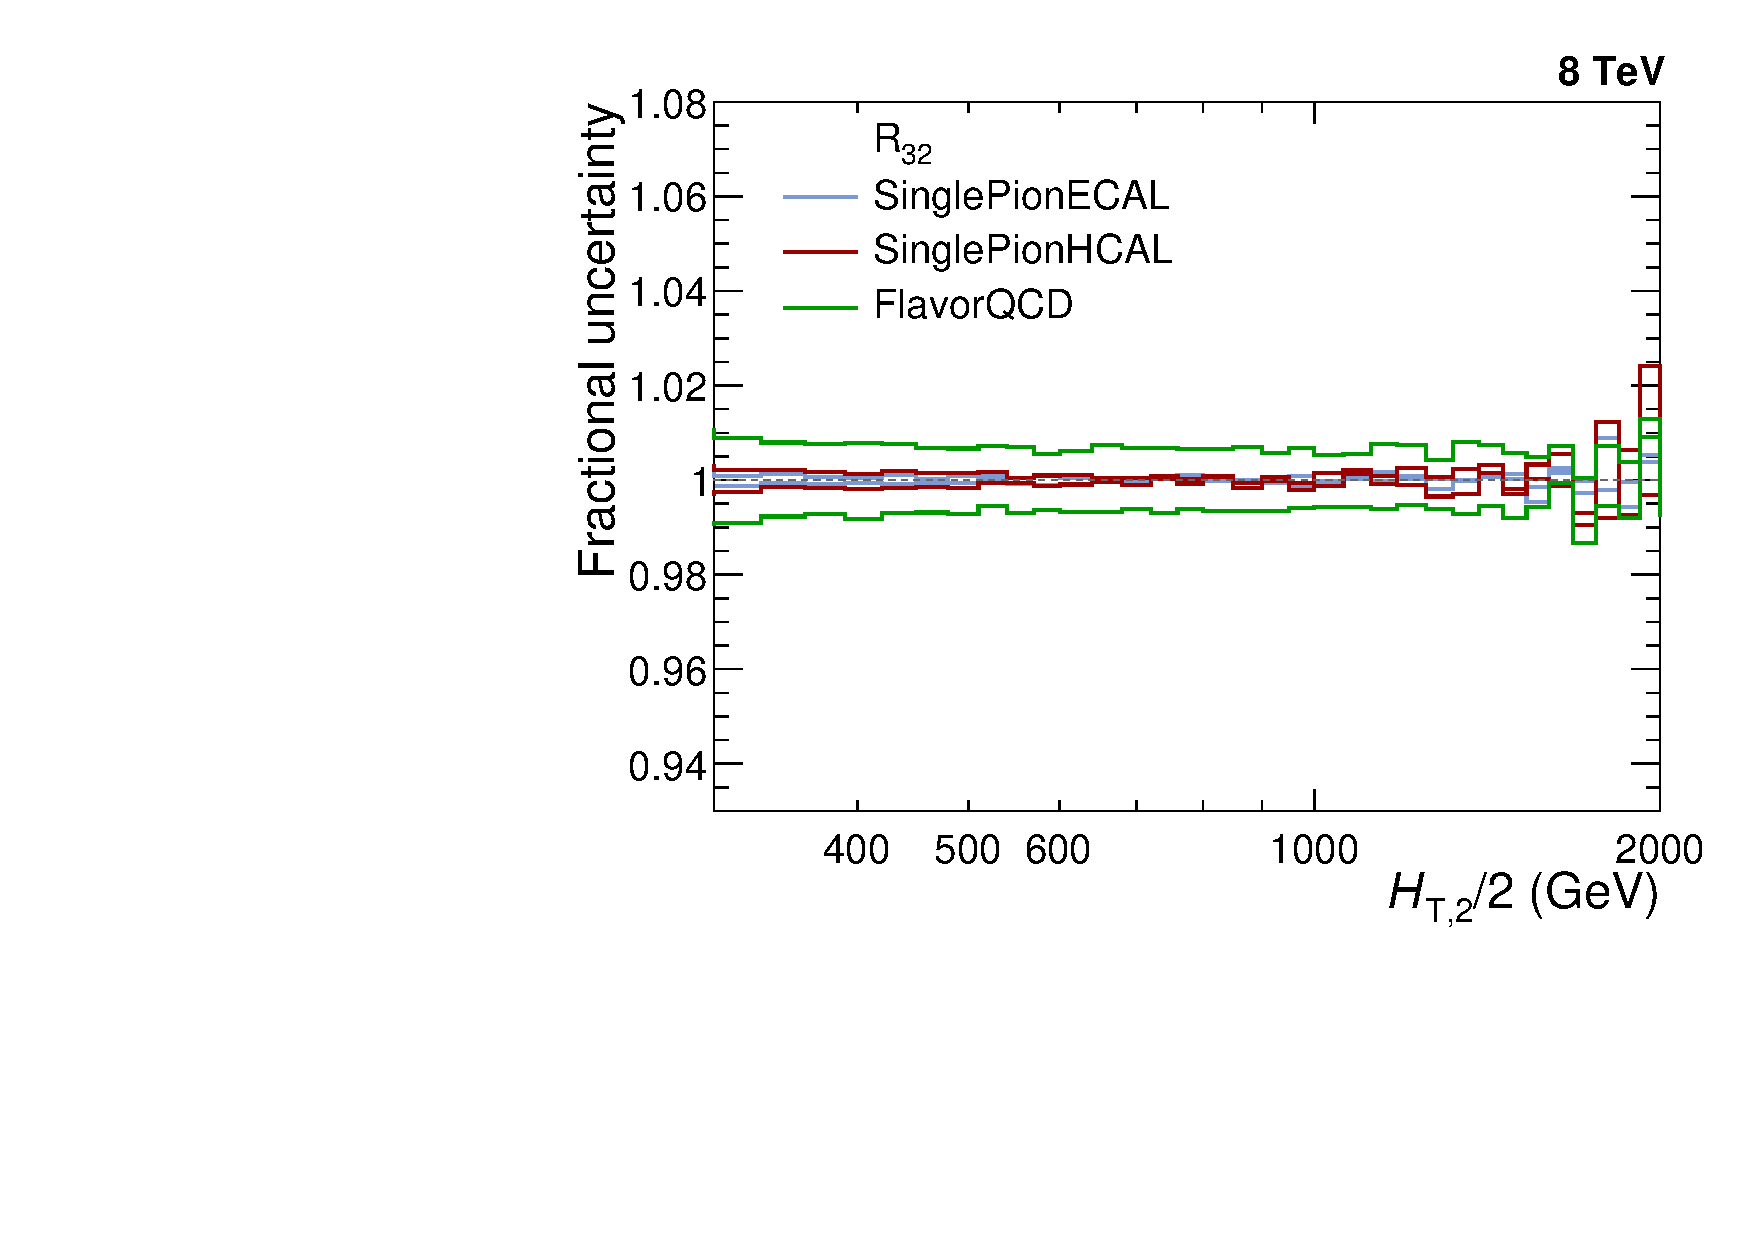
\includegraphics[width=0.51\textwidth]{/home/anter/Desktop/Thesis/Plots_HT_2_150/Single/MC_Macro_Plot_Ratio_32_HT_2_Unc_Single_1.pdf}\\
\caption{The relative size of the jet energy correction (JEC) uncertainties for individual sources are shown for inclusive 2-jet (top) and 3-jet events cross sections (middle) and cross section ratio \ratio (bottom). On left, JEC uncertainties are evaluated from \textcolor{blue2}{AbsoluteStat}, \textcolor{red}{AbsoluteScale}, \textcolor{green}{AbsoluteMPFBias} and \textcolor{pink2}{Fragmentation} sources whereas on right, these are evaluated from \textcolor{blue2}{SinglePionECAL}, \textcolor{red}{SinglePionHCAL} and \textcolor{green}{FlavorQCD} sources.}
\label{fig:jes1}
%\end{center}
\end{figure}

\begin{figure}[!hbtp]
%\begin{center}
\hspace*{-5mm}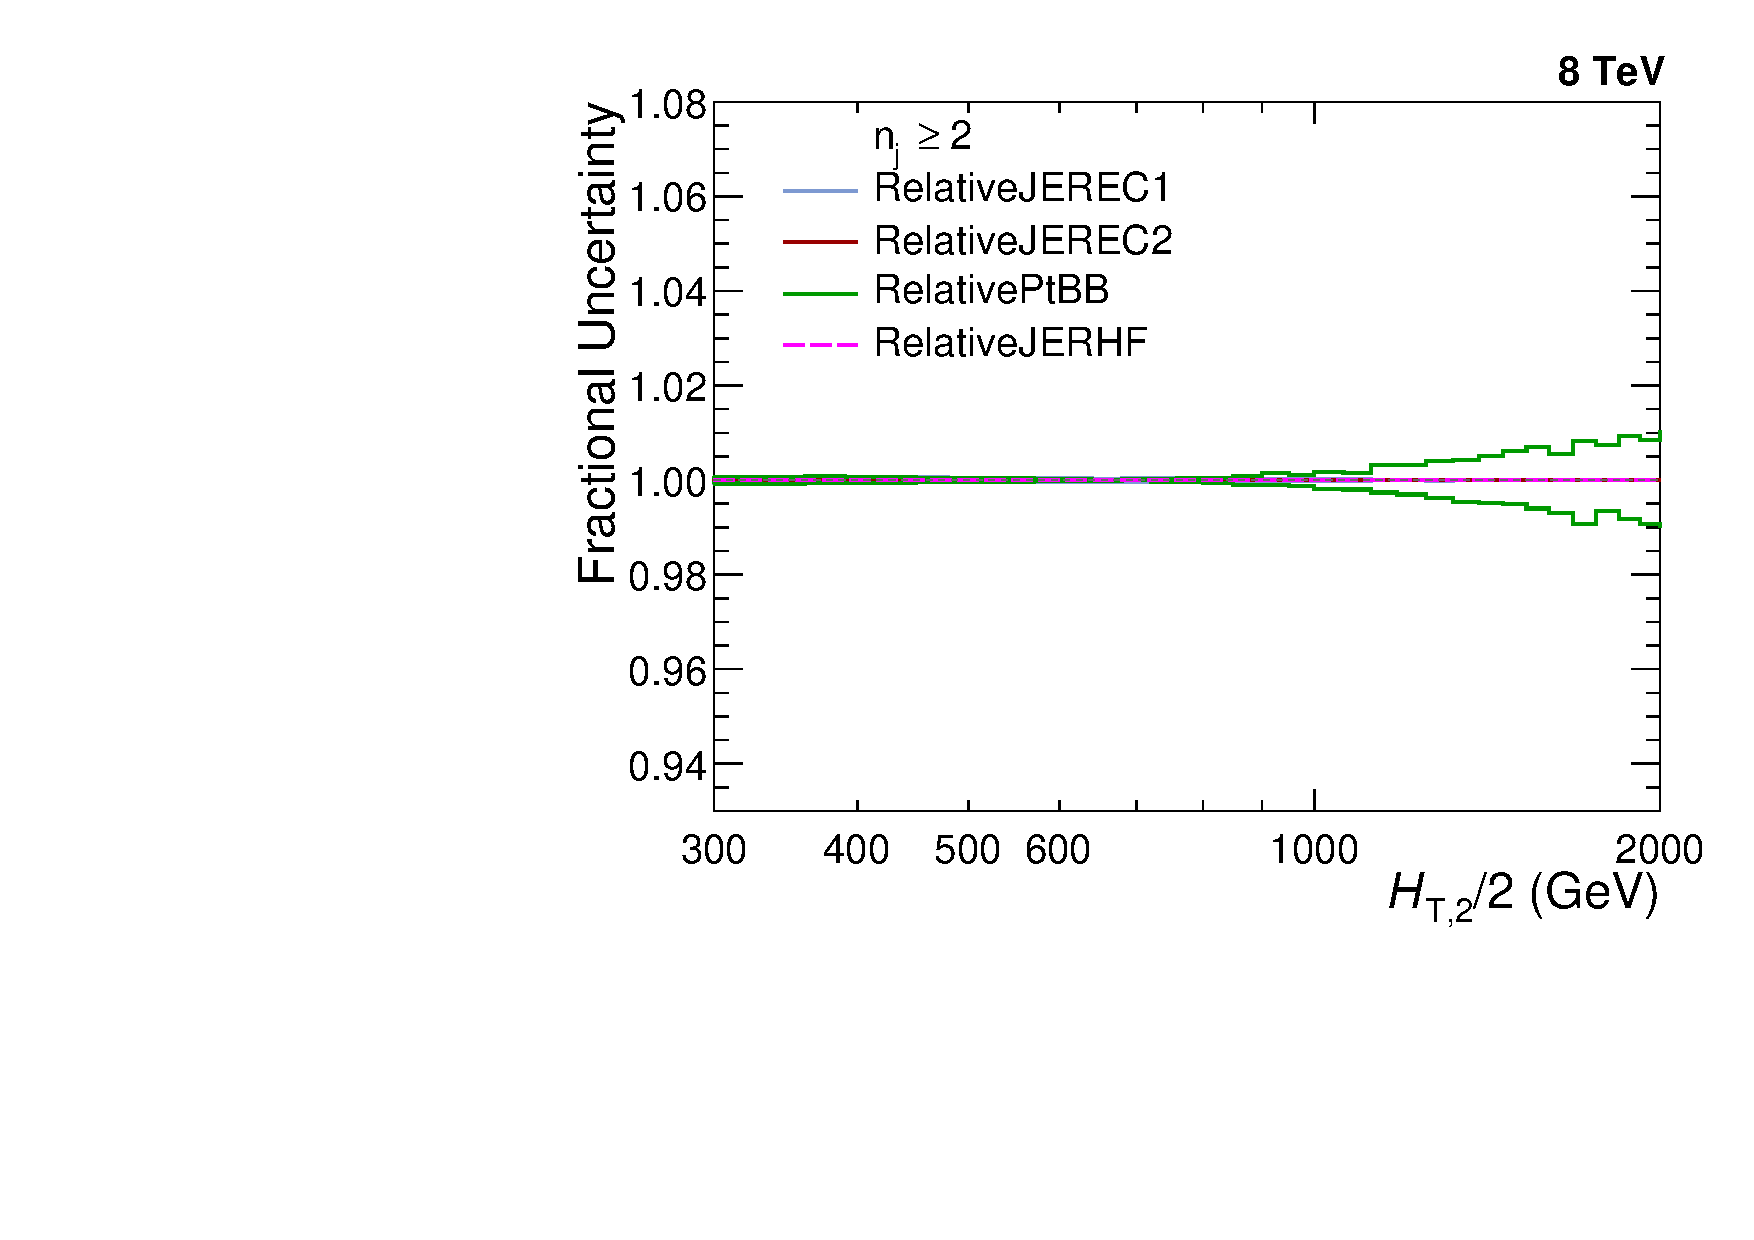
\includegraphics[width=0.51\textwidth]{/home/anter/Desktop/Thesis/Plots_HT_2_150/Single/MC_Macro_Plot_All_2_HT_2_Unc_Relative_1.pdf}%
~~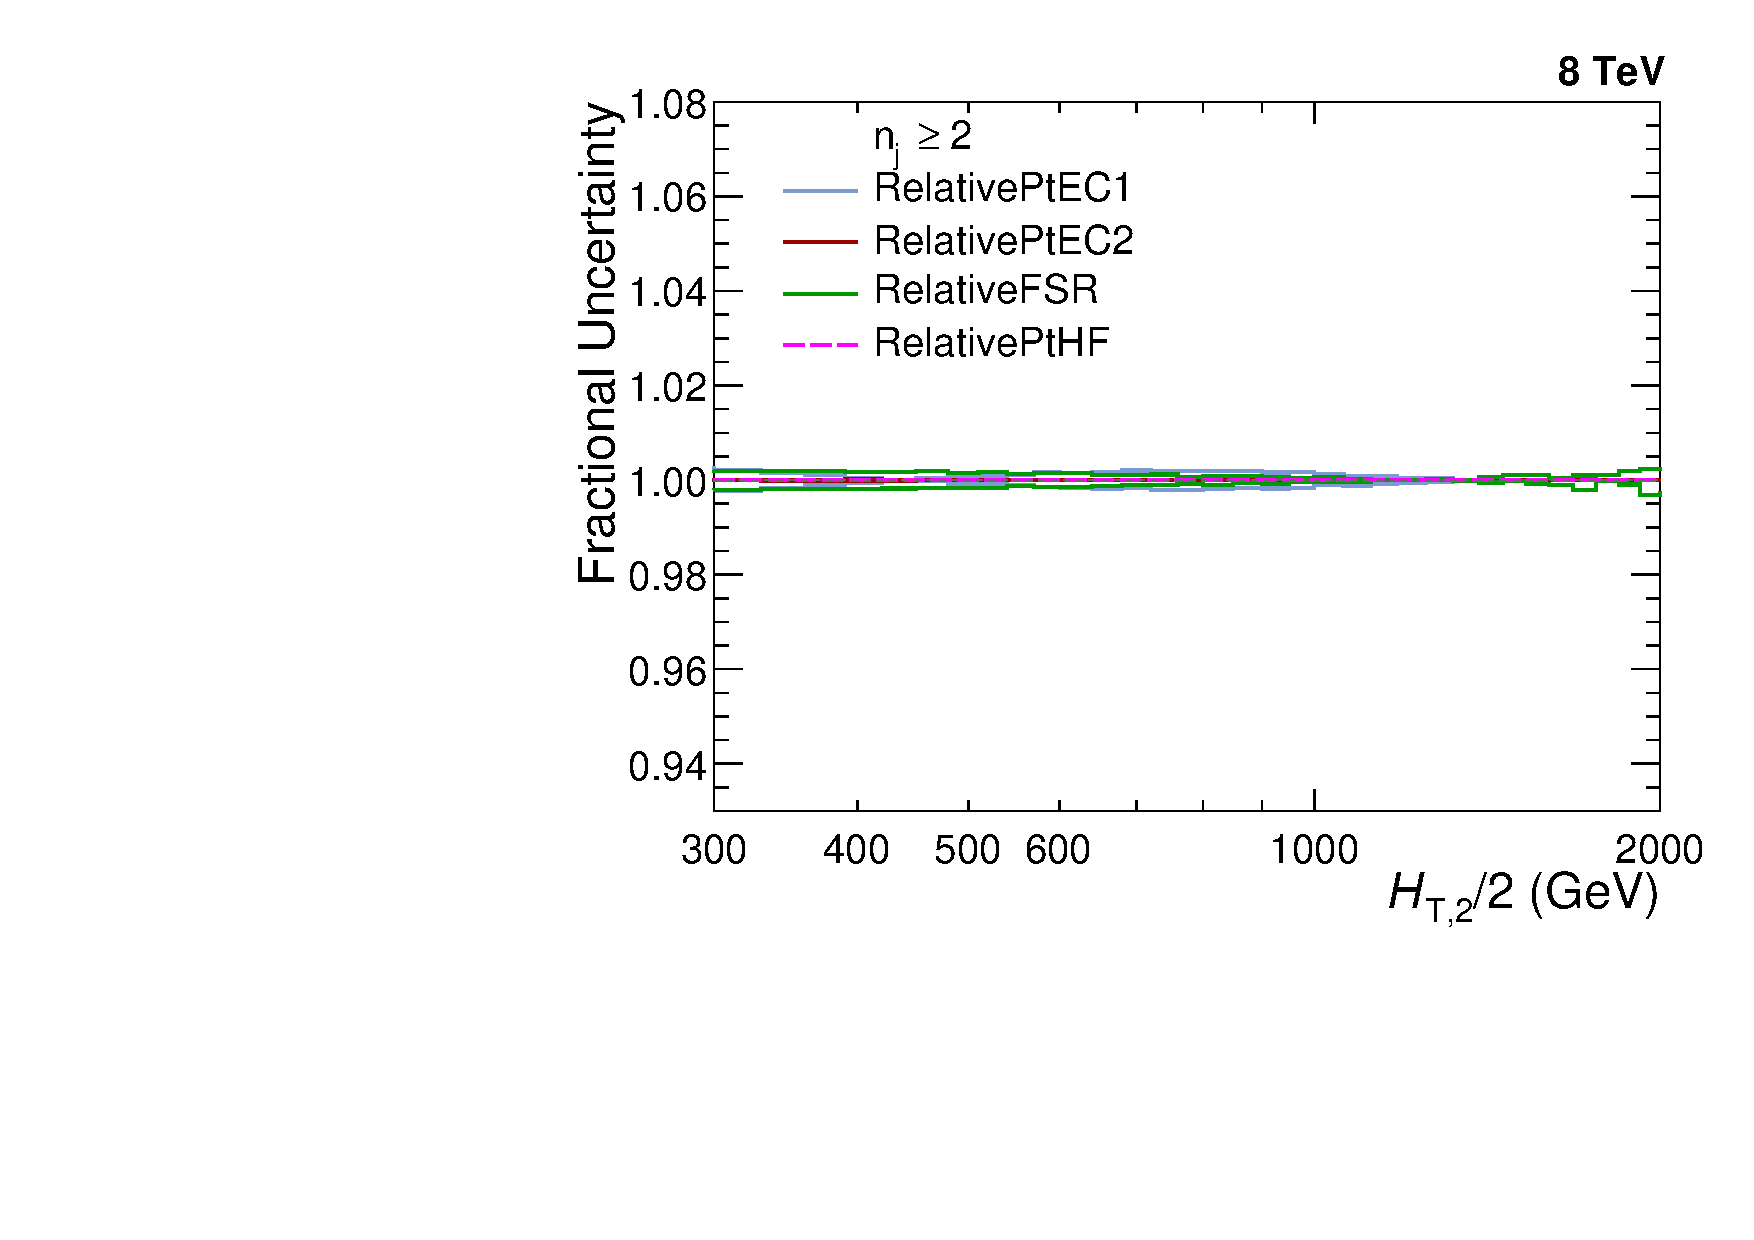
\includegraphics[width=0.51\textwidth]{/home/anter/Desktop/Thesis/Plots_HT_2_150/Single/MC_Macro_Plot_All_2_HT_2_Unc_Relative_2.pdf}\\
\hspace*{-5mm}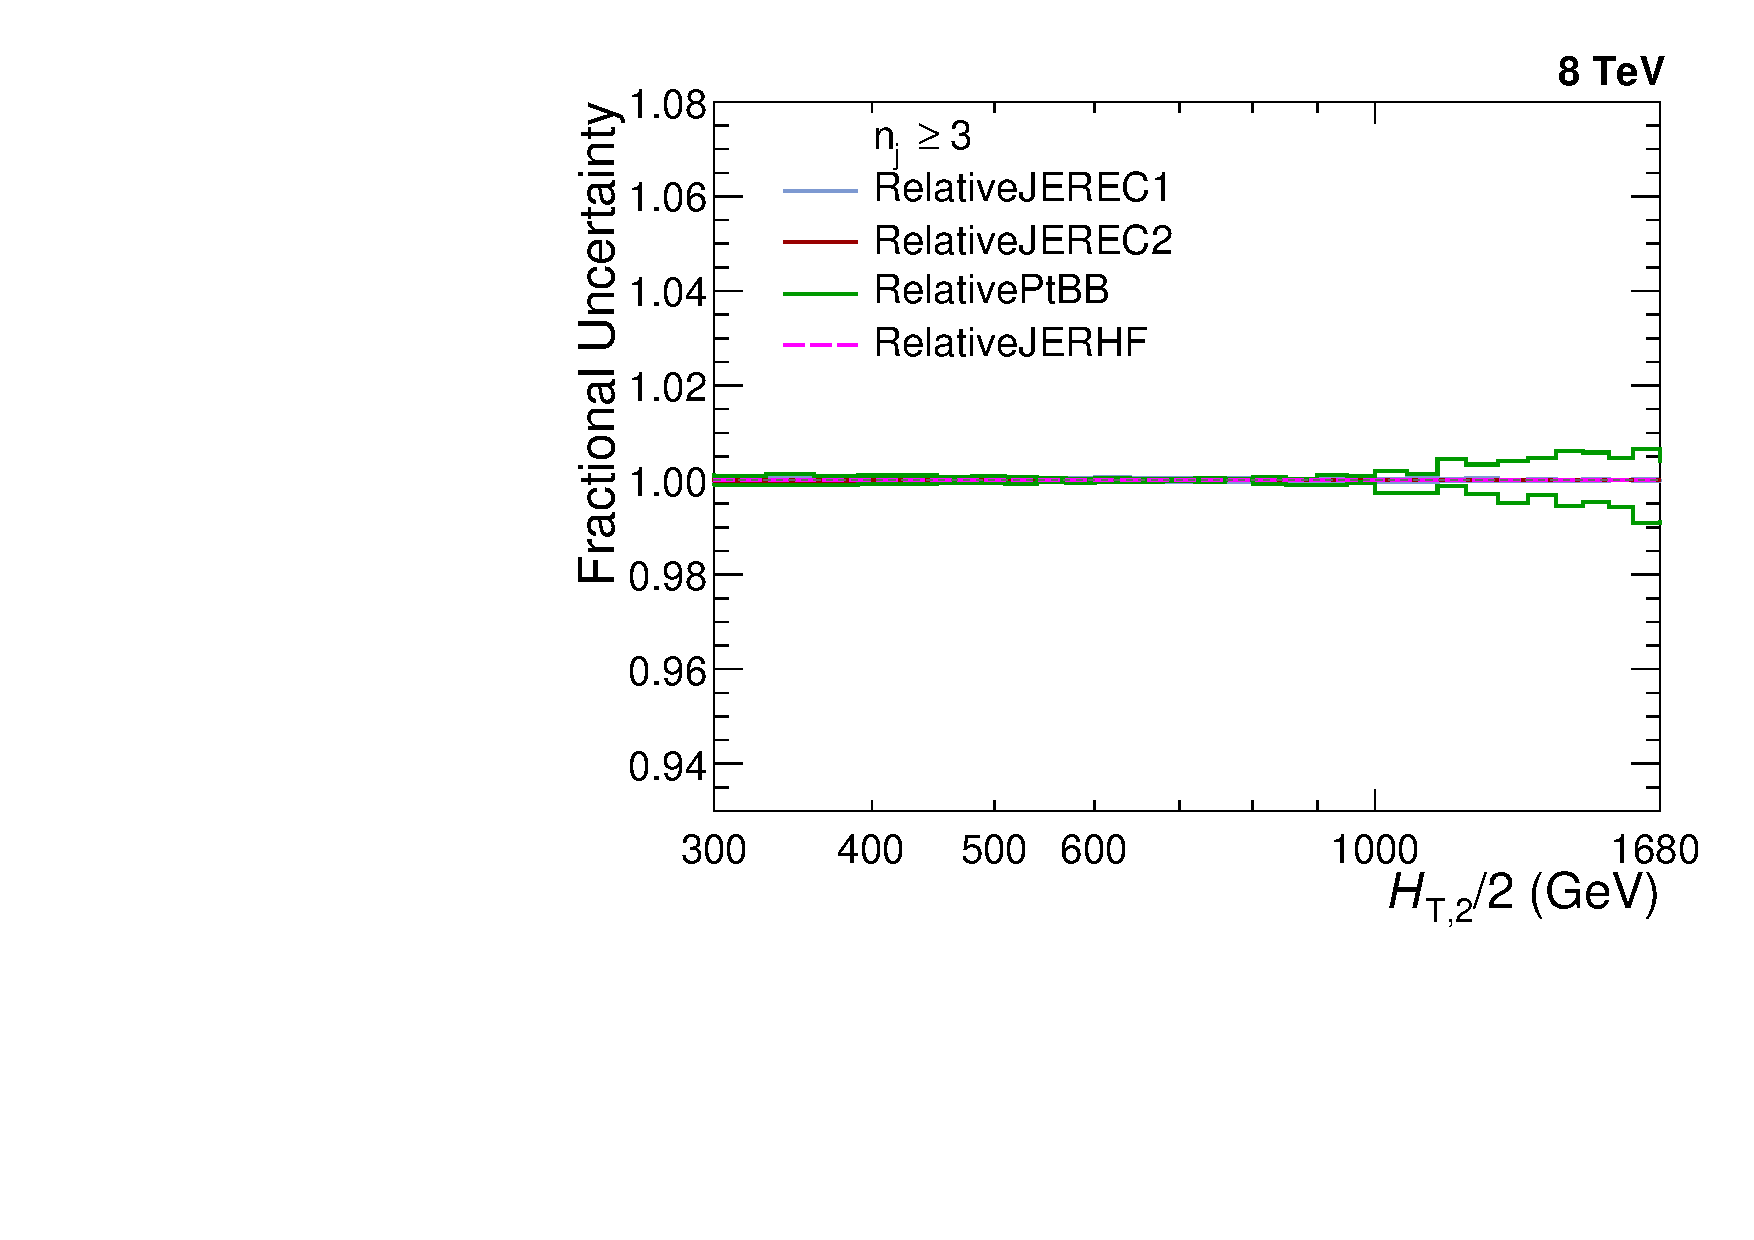
\includegraphics[width=0.51\textwidth]{/home/anter/Desktop/Thesis/Plots_HT_2_150/Single/MC_Macro_Plot_All_3_HT_2_Unc_Relative_1.pdf}%
~~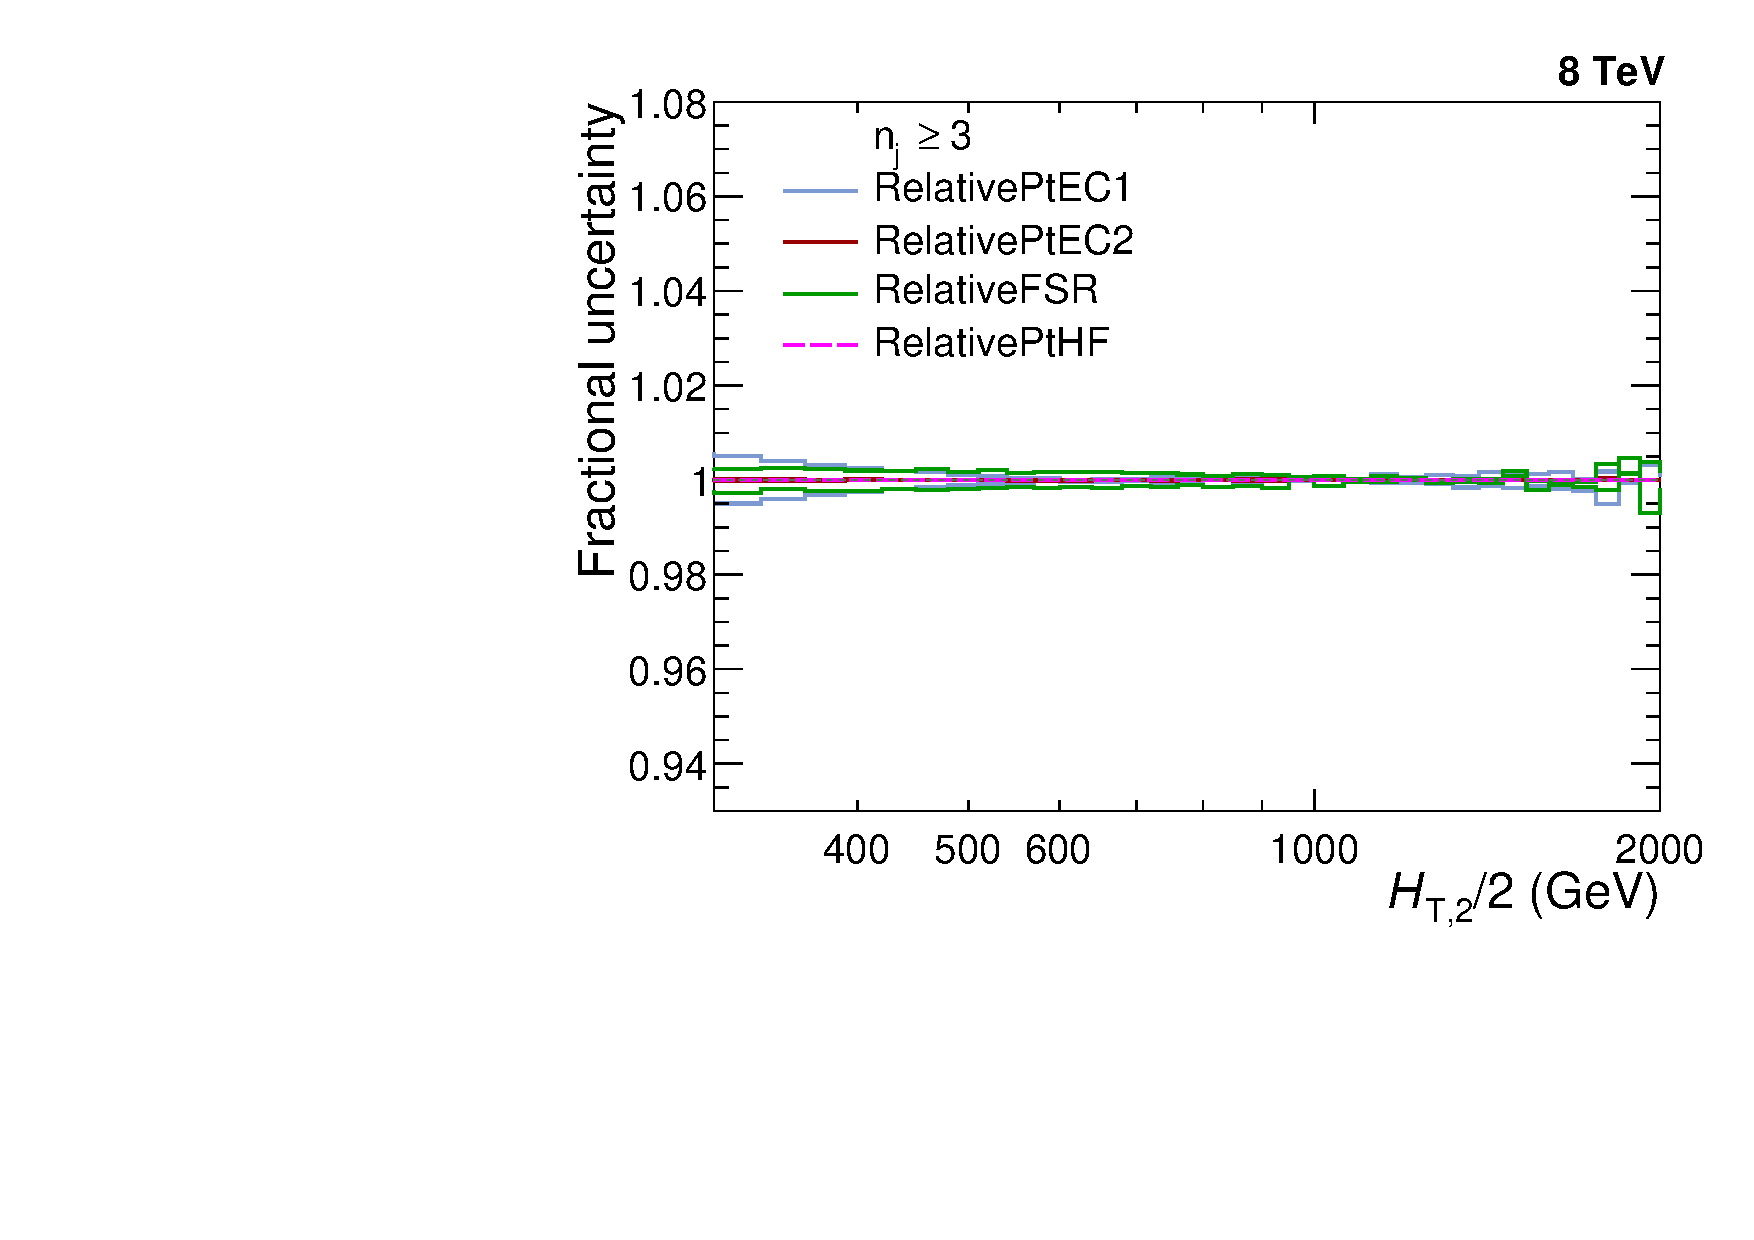
\includegraphics[width=0.51\textwidth]{/home/anter/Desktop/Thesis/Plots_HT_2_150/Single/MC_Macro_Plot_All_3_HT_2_Unc_Relative_2.pdf}\\
\hspace*{-5mm}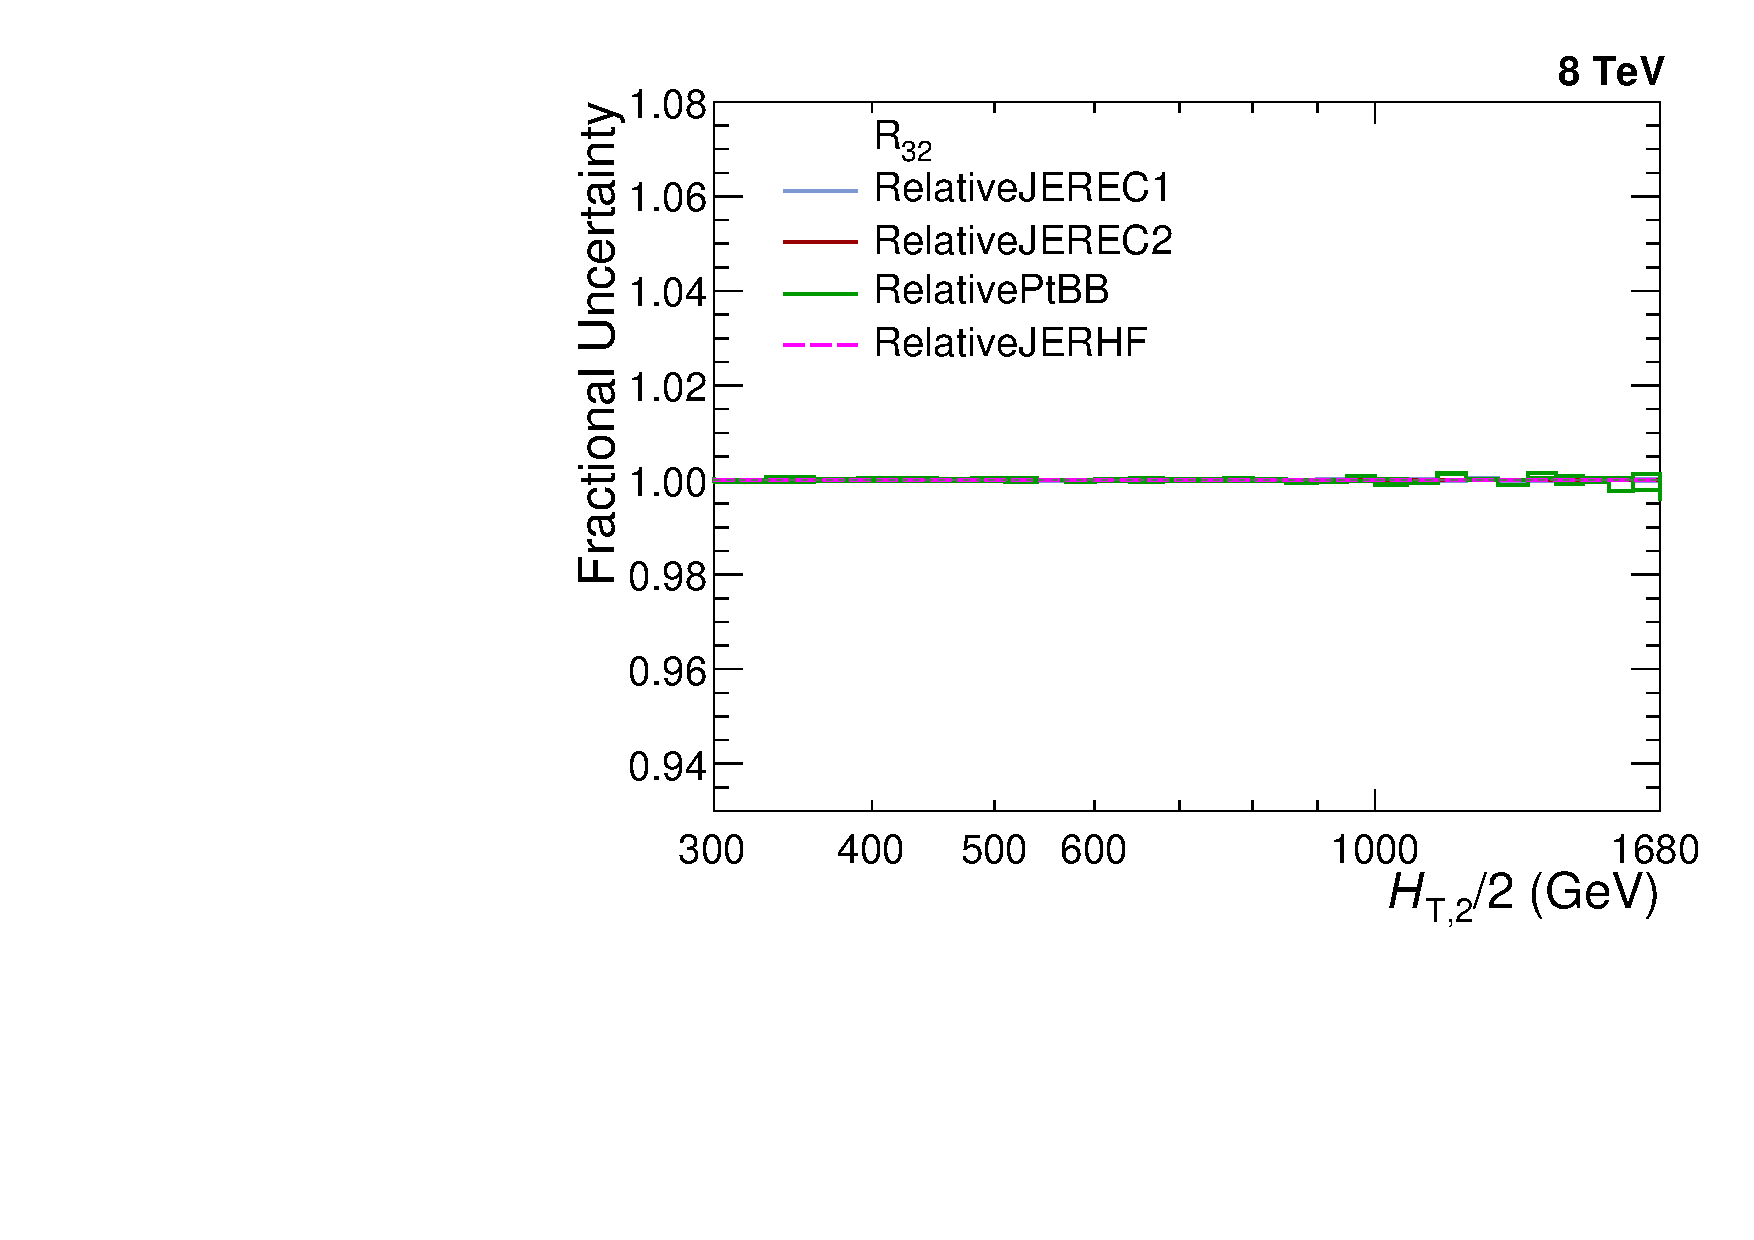
\includegraphics[width=0.51\textwidth]{/home/anter/Desktop/Thesis/Plots_HT_2_150/Single/MC_Macro_Plot_Ratio_32_HT_2_Unc_Relative_1.pdf}%
~~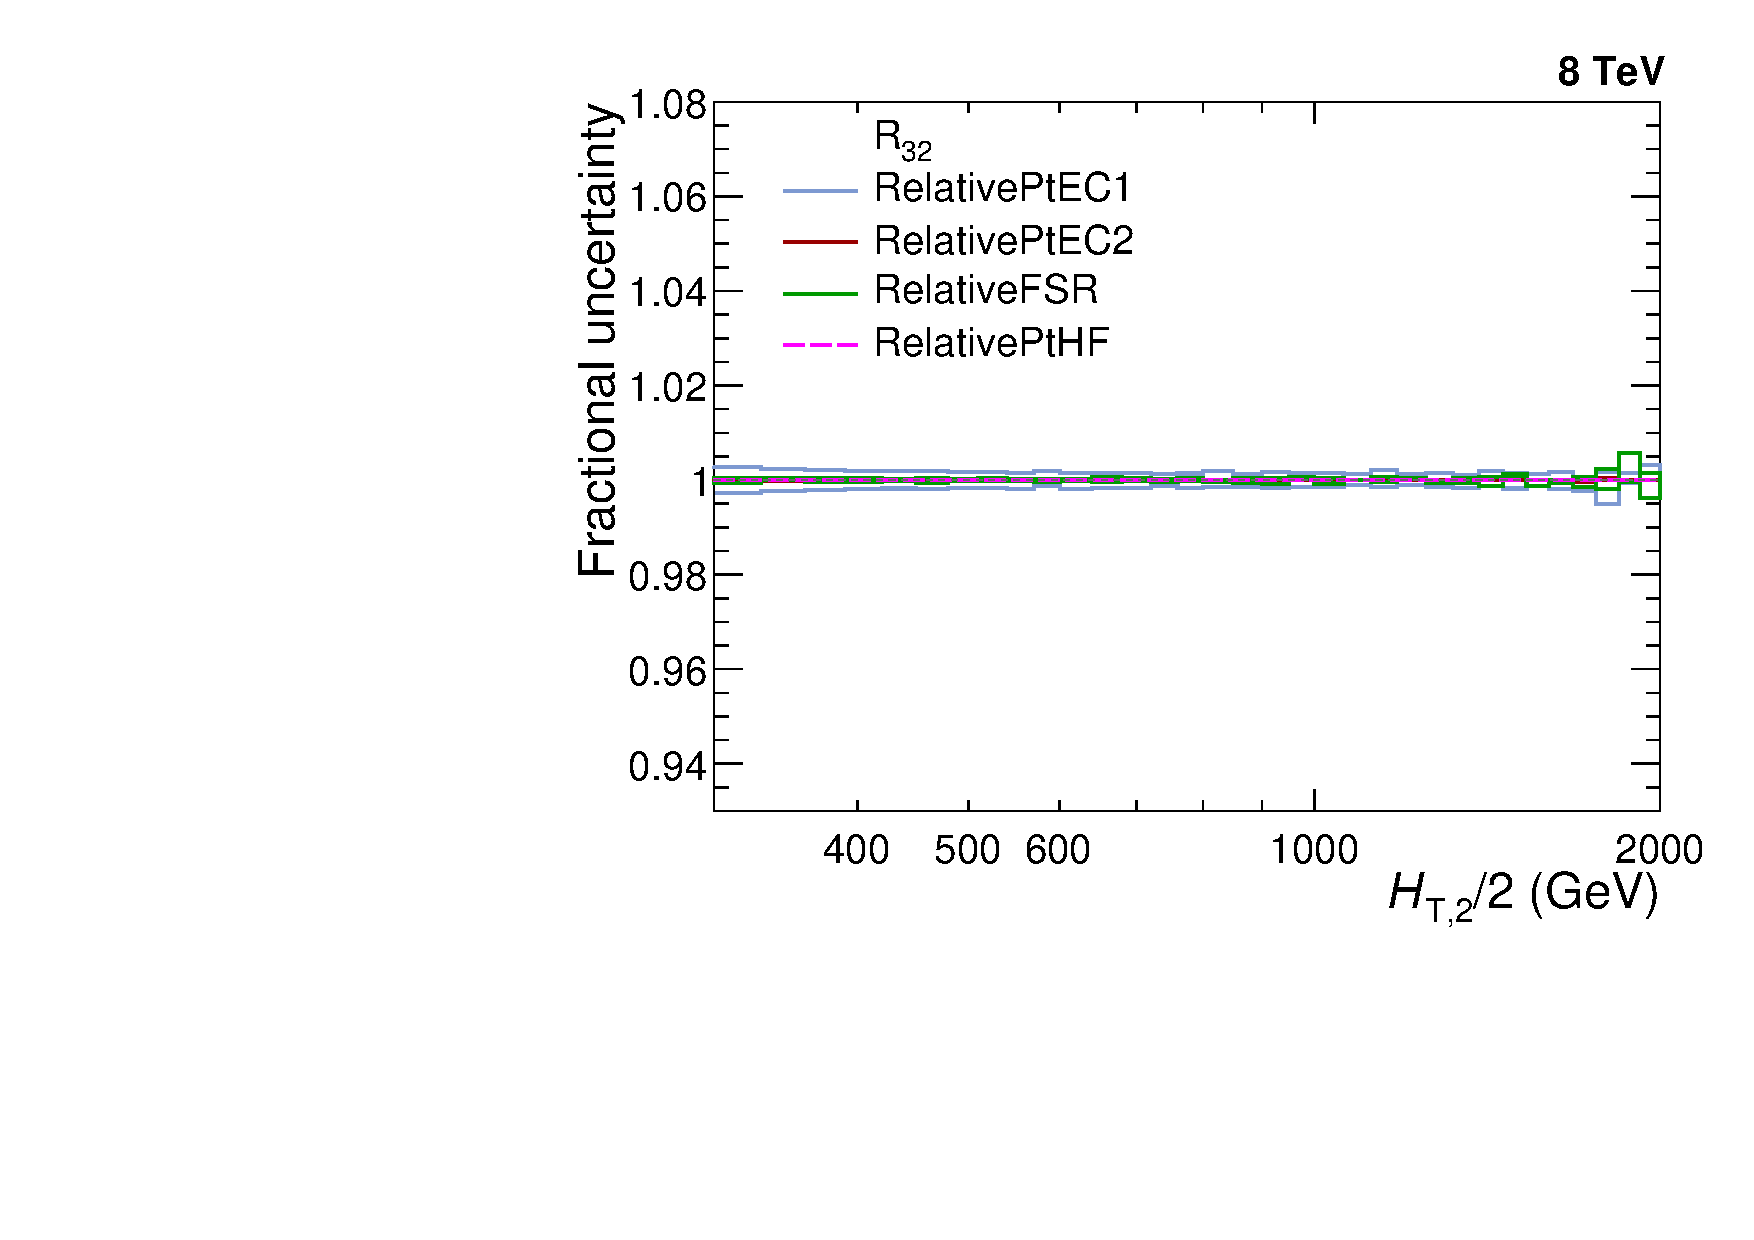
\includegraphics[width=0.51\textwidth]{/home/anter/Desktop/Thesis/Plots_HT_2_150/Single/MC_Macro_Plot_Ratio_32_HT_2_Unc_Relative_2.pdf}\\
\caption{The relative size of the jet energy correction (JEC) uncertainties for individual sources are shown for inclusive 2-jet (top) and 3-jet events cross sections (middle) and cross section ratio \ratio (bottom). On left, JEC uncertainties are evaluated from \textcolor{blue2}{RelativeJEREC1}, \textcolor{red}{RelativeJEREC2}, \textcolor{green}{RelativePtBB} and \textcolor{pink2}{RelativeJERHF} sources whereas on right, these are evaluated from \textcolor{blue2}{RelativePtEC1}, \textcolor{red}{RelativePtEC2}, \textcolor{green}{RelativePFSR} and \textcolor{pink2}{RelativePtHF} sources.}
\label{fig:jes2}
%\end{center}
\end{figure}

\begin{figure}[!hbtp]
%\begin{center}
\hspace*{-5mm}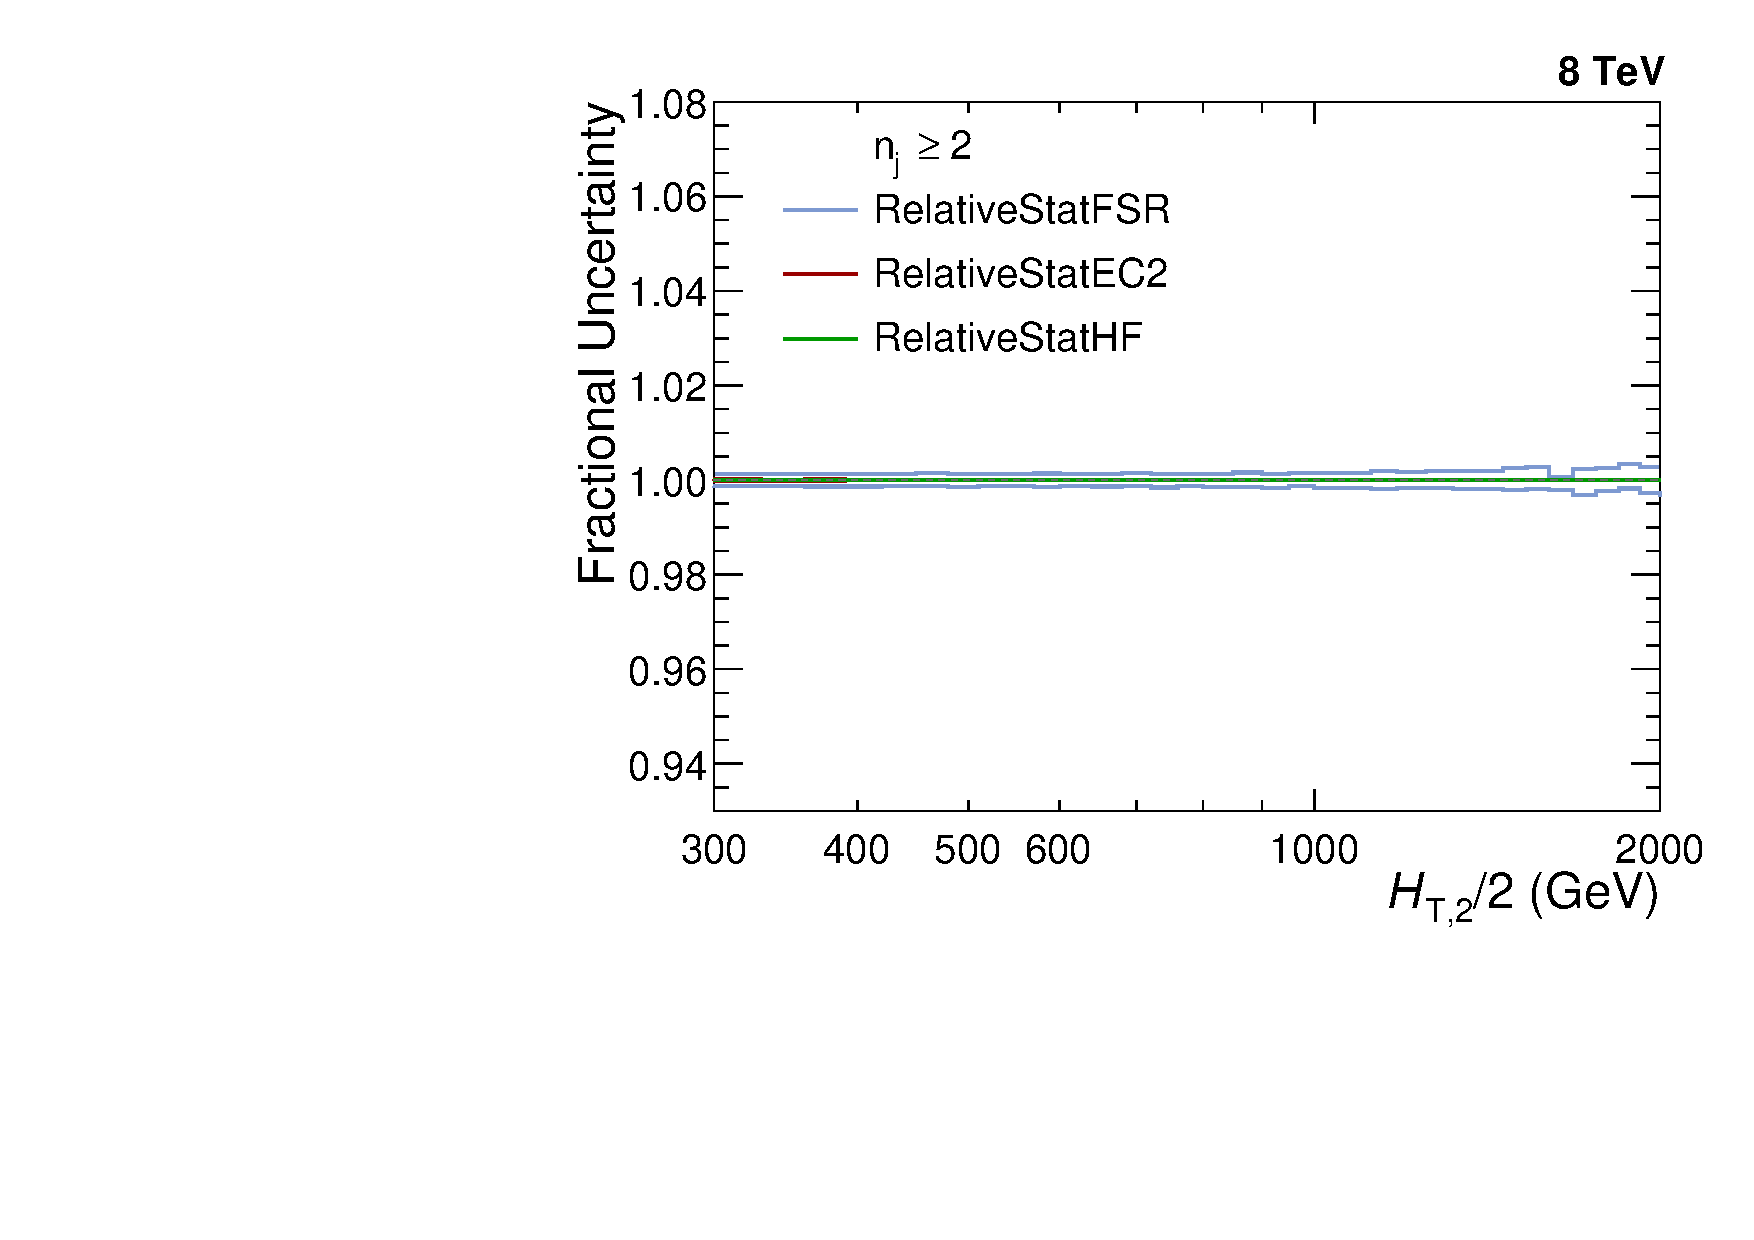
\includegraphics[width=0.51\textwidth]{/home/anter/Desktop/Thesis/Plots_HT_2_150/Single/MC_Macro_Plot_All_2_HT_2_Unc_RelativeStat_1.pdf}%
~~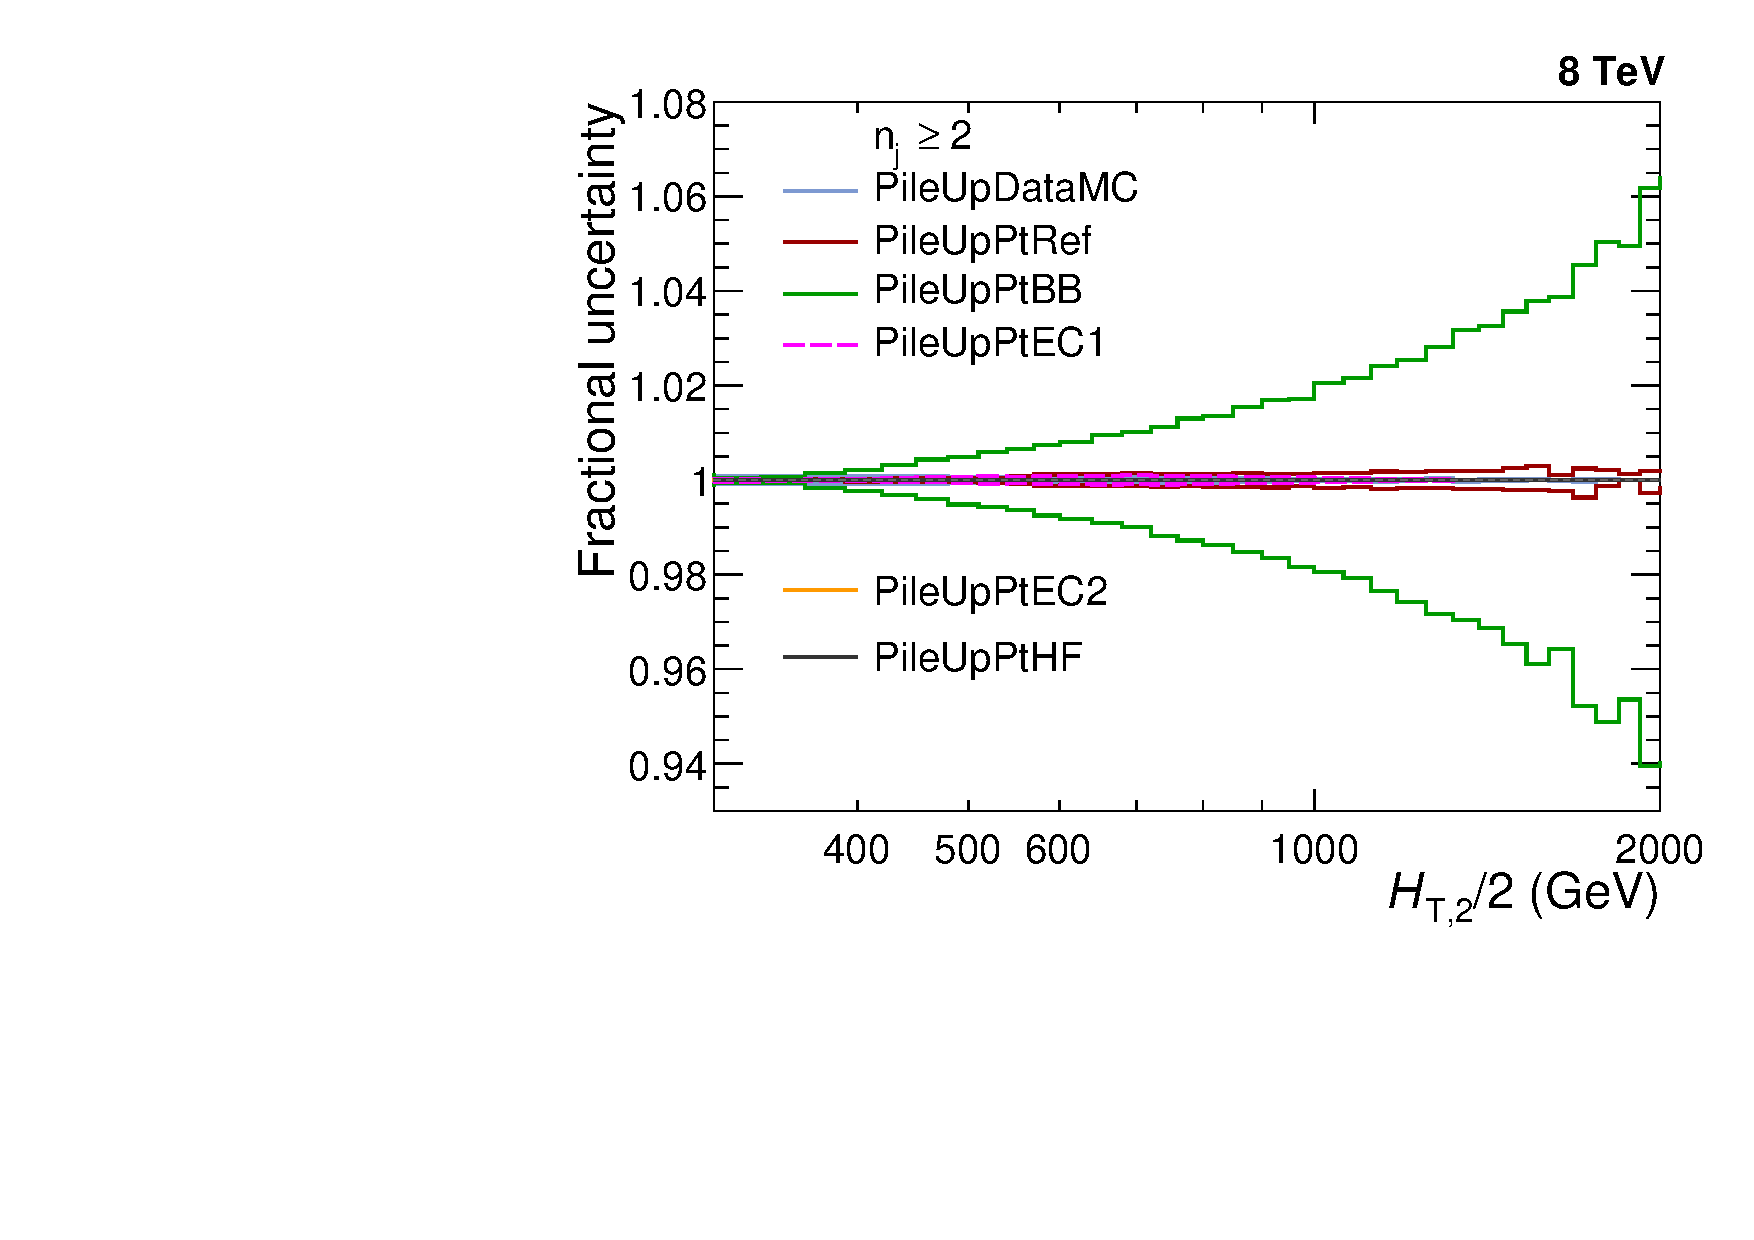
\includegraphics[width=0.51\textwidth]{/home/anter/Desktop/Thesis/Plots_HT_2_150/Single/MC_Macro_Plot_All_2_HT_2_Unc_Pileup_1.pdf}\\
\hspace*{-5mm}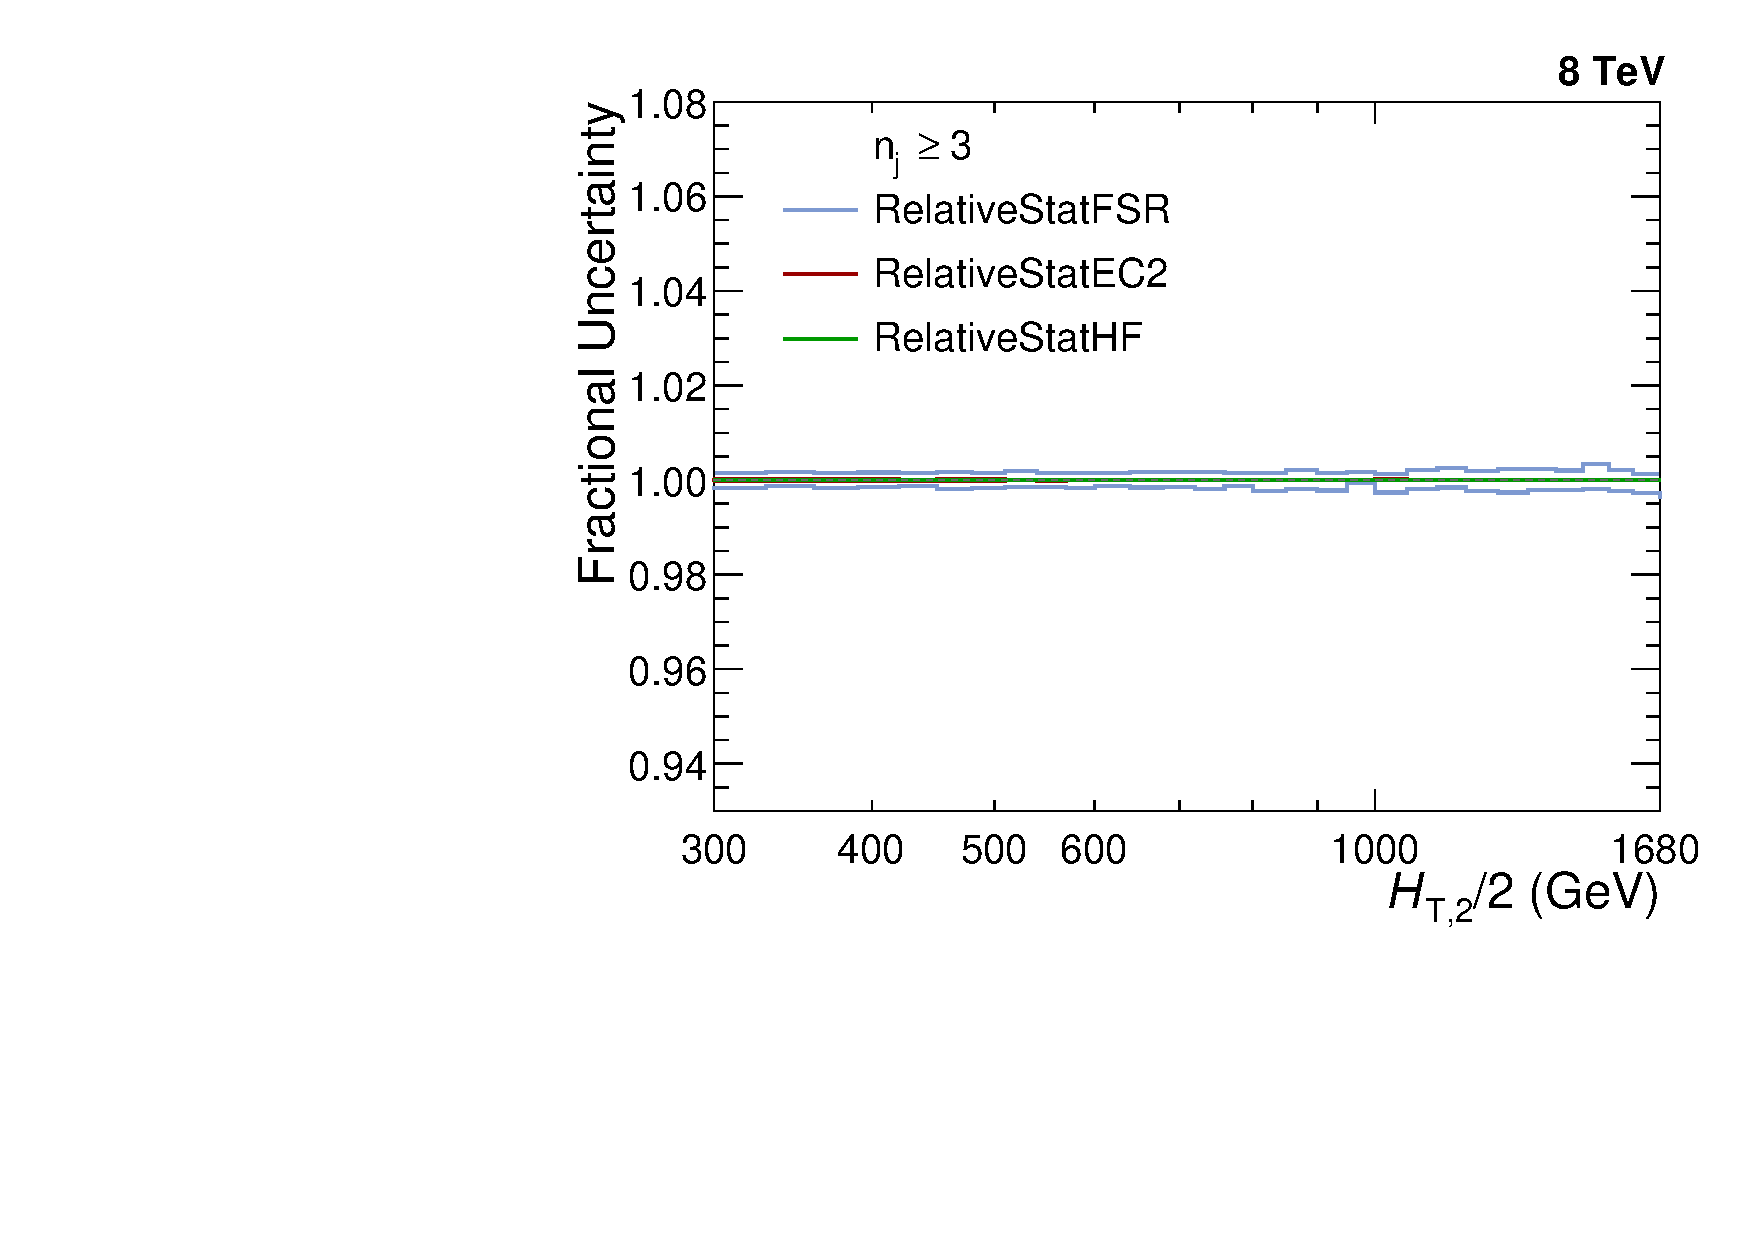
\includegraphics[width=0.51\textwidth]{/home/anter/Desktop/Thesis/Plots_HT_2_150/Single/MC_Macro_Plot_All_3_HT_2_Unc_RelativeStat_1.pdf}%
~~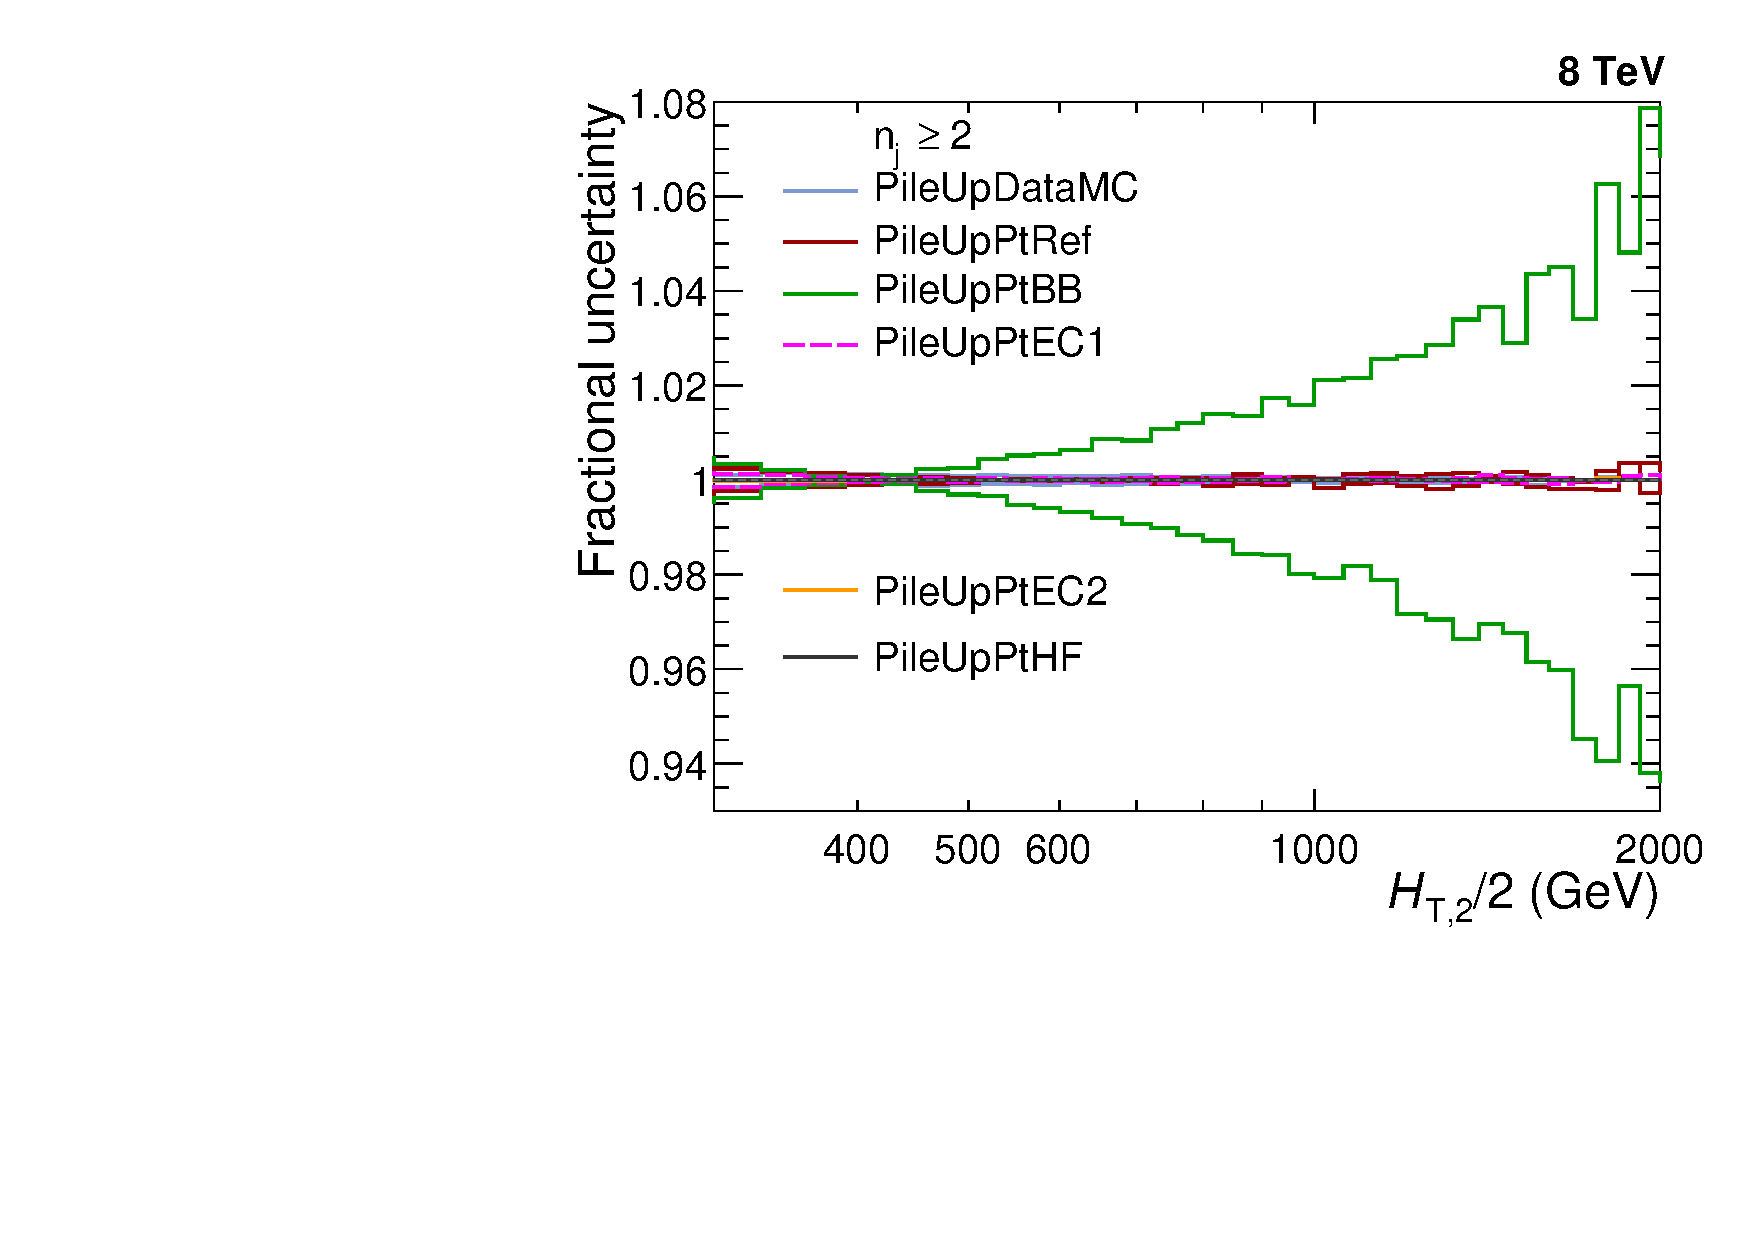
\includegraphics[width=0.51\textwidth]{/home/anter/Desktop/Thesis/Plots_HT_2_150/Single/MC_Macro_Plot_All_3_HT_2_Unc_Pileup_1.pdf}\\
\hspace*{-5mm}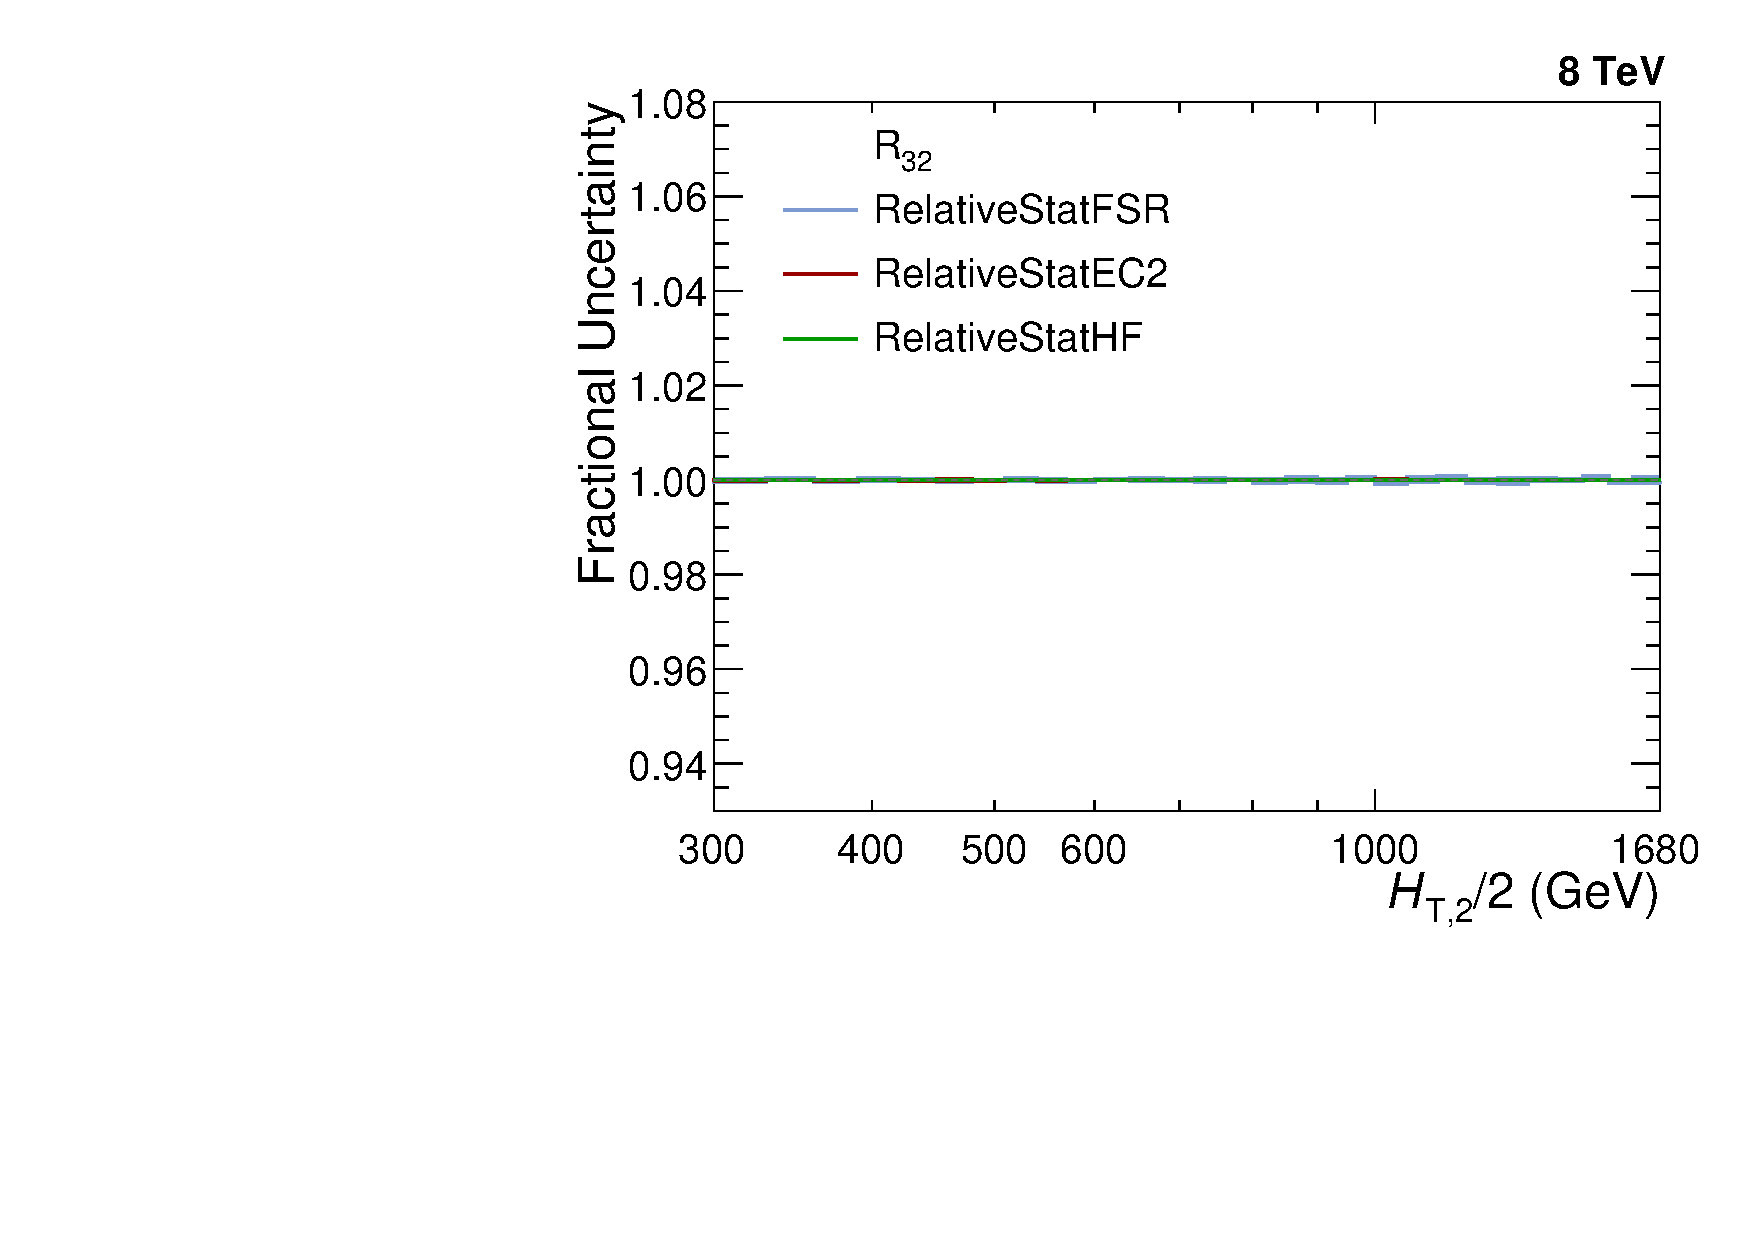
\includegraphics[width=0.51\textwidth]{/home/anter/Desktop/Thesis/Plots_HT_2_150/Single/MC_Macro_Plot_Ratio_32_HT_2_Unc_RelativeStat_1.pdf}%
~~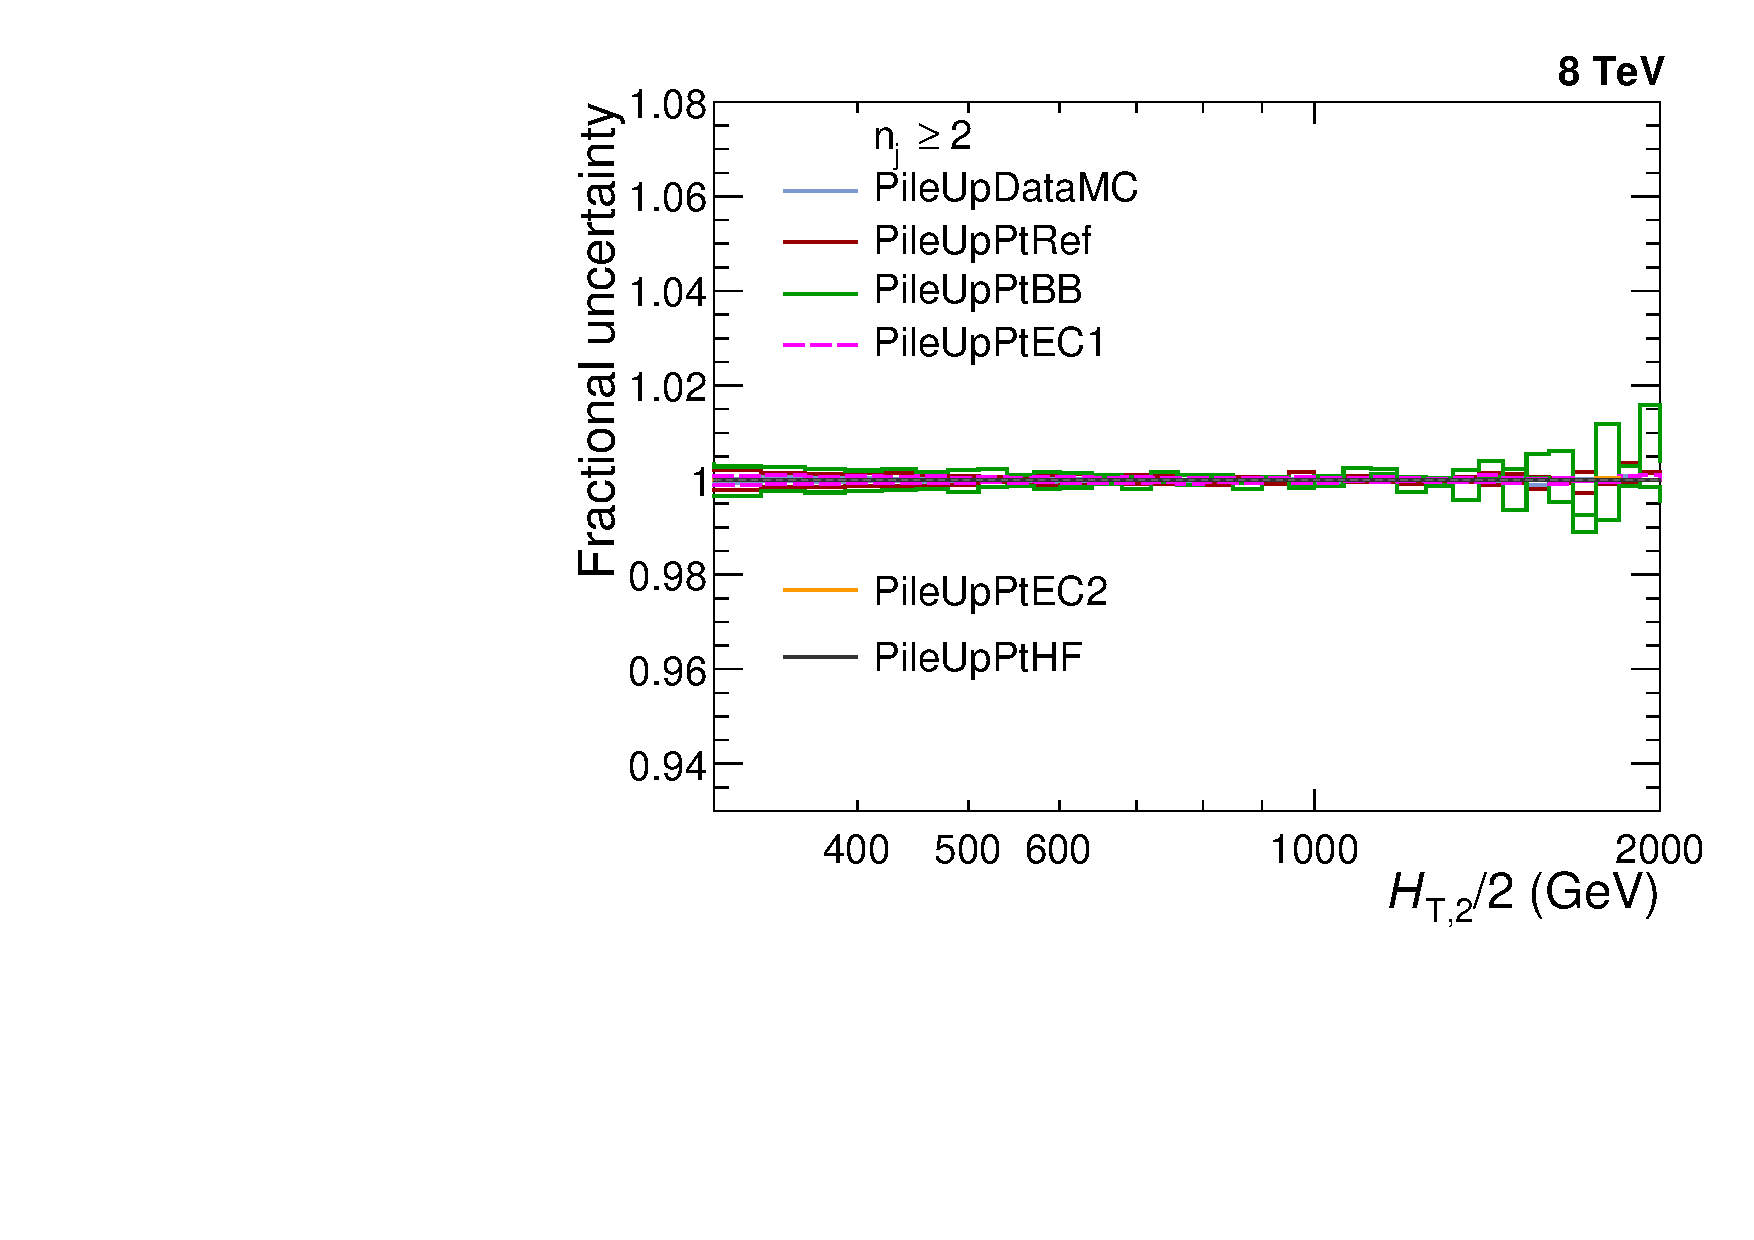
\includegraphics[width=0.51\textwidth]{/home/anter/Desktop/Thesis/Plots_HT_2_150/Single/MC_Macro_Plot_Ratio_32_HT_2_Unc_Pileup_1.pdf}\\
\caption{The relative size of the jet energy correction (JEC) uncertainties for individual sources are shown for inclusive 2-jet (top) and 3-jet events cross sections (middle) and cross section ratio \ratio (bottom). On left, JEC uncertainties are evaluated from \textcolor{blue2}{RelativeStatFSR}, \textcolor{red}{RelativeStatEC2} and \textcolor{green}{RelativeStatHF} sources whereas on right, these are evaluated from \textcolor{blue2}{PileUpDataMC}, \textcolor{red}{PileUpPtRef}, \textcolor{green}{PileUpPtBB}, \textcolor{pink2}{PileUpPtEC1}, \textcolor{deepsaffron}{PileUpPtEC2} and \textcolor{dimgray}{PileUpPtHF} sources.}
\label{fig:jes3}
%\end{center}
\end{figure}

